% 技术文档（官方模板结构）。数字一律来自双花括号事实占位，由 build_submission.py 渲染后用 latexmk -xelatex 编译。
\documentclass[zihao=-4,a4paper,fontset=none,linespread=1.3]{ctexart}

% ---------------------------------------------------------------- 版式：与官方 docx 模板一致
\usepackage[left=3.17cm,right=3.17cm,top=3.2cm,bottom=2.54cm,headsep=0.8cm,footskip=1.0cm]{geometry}
\usepackage{fontspec}
\setmainfont{TeX Gyre Termes}                      % Times New Roman 的开源等价字体
\setsansfont{TeX Gyre Heros}
\setmonofont{Latin Modern Mono}[Scale=0.95]
\setCJKmainfont{FandolSong-Regular}[BoldFont=FandolSong-Bold,ItalicFont=FandolKai-Regular]   % 宋体
\setCJKsansfont{FandolHei-Regular}[BoldFont=FandolHei-Bold]                                  % 黑体
\setCJKmonofont{FandolFang-Regular}

\usepackage{graphicx,booktabs,tabularx,multirow,array,float,xcolor,enumitem,amsmath,pifont}
\usepackage[font=small,labelsep=quad]{caption}
\usepackage{tikz}
\usetikzlibrary{arrows.meta,positioning,fit,backgrounds,calc,shapes.geometric}
\usepackage[hidelinks,bookmarksnumbered]{hyperref}
\usepackage{fancyhdr}
\pagestyle{fancy}\fancyhf{}\renewcommand{\headrulewidth}{0pt}\cfoot{\small\thepage}
\fancypagestyle{plain}{\fancyhf{}\renewcommand{\headrulewidth}{0pt}\cfoot{\small\thepage}}

\graphicspath{{figures/}{../../metrics/evidence/}{../../metrics/evidence/figures/}{../../metrics/evidence/screenshots/}}

% 页眉原图提取自官方《技术文档模板.docx》；保持564:103原图比例。
% 参照模板渲染坐标：居中、顶边42.5bp、宽184.7bp，细线y=77.7bp。
\AddToHook{shipout/background}{%
  \begin{tikzpicture}[remember picture,overlay]
    \node[anchor=north,inner sep=0pt,outer sep=0pt]
      at ([yshift=-42.5bp]current page.north)
      {
\includegraphics[width=184.7bp]{figures/official_header.png}};
    \draw[line width=0.75bp]
      ([xshift=3.17cm,yshift=-77.7bp]current page.north west) --
      ([xshift=-3.17cm,yshift=-77.7bp]current page.north east);
  \end{tikzpicture}%
}


% 章：第一部分 作品概述（四号加粗黑体）；节 1.1、小节 2.2.1（小四加粗）
\ctexset{
  section={name={第,部分},number=\chinese{section},format=\zihao{4}\sffamily\bfseries,aftername=\quad,beforeskip=1.6ex plus .3ex,afterskip=1.0ex},
  subsection={format=\zihao{-4}\sffamily\bfseries,beforeskip=1.2ex plus .2ex,afterskip=.6ex},
  subsubsection={format=\zihao{-4}\sffamily\bfseries,beforeskip=1.0ex,afterskip=.4ex},
  appendix={name={附录},number=\Alph{section}},
}
\renewcommand{\thesubsection}{\arabic{section}.\arabic{subsection}}
\setlist{nosep,leftmargin=2em}
\setlength{\parindent}{2em}
\renewcommand{\arraystretch}{1.25}

% 常用记号
\newcommand{\doccite}[1]{\textsuperscript{[\ref{#1}]}}
\newcommand{\ms}{\,ms}
\newcommand{\us}{\,\textmu s}
\newcommand{\pending}{\textbf{【待补充指标】}}
\newcommand{\figplaceholder}[2]{\fbox{\parbox[c][#2][c]{0.9\linewidth}{\centering\color{gray}#1}}}
\newcolumntype{Y}{>{\raggedright\arraybackslash}X}
\newcolumntype{C}{>{\centering\arraybackslash}X}

\begin{document}

\begin{center}
  {\zihao{-2}\sffamily\bfseries 异构协同具身智能机械臂控制系统}
\end{center}
\vspace{0.5ex}

\noindent{\zihao{4}\sffamily\bfseries 摘要}
\vspace{0.6ex}

面向小零件配料与分拣，本作品设计了一套由 AMD Ryzen AI PC、Kria KV260 和六轴机械臂组成的桌面分拣系统。用户输入中文指令，指定零件类别、数量和目标托盘，系统依次完成指令解析、目标识别、轨迹规划、抓取放置与结果核验。作品以 M12、M6 螺丝和螺母为操作对象，任务执行不依赖云端推理。

AI PC 负责感知与规划：YOLO11n-seg 实例分割模型经 Quark A8W8 量化后部署在 NPU，本地 Qwen2.5-VL-3B 在 GPU 上辅助解析指令并复核结果，CPU 完成坐标变换和轨迹规划。KV260 负责执行与腕部纠偏：ARM 处理器运行作业管理和视觉定位，FPGA 可编程逻辑（PL）完成 5\ms 轨迹求值、CAN 调度、执行保护和在线修正，大螺丝的腕部图像掩码由 PL 加速。头部相机提供整盘目标位置，腕部相机在抓取前校正局部偏差，放置后再由头部相机核验结果。

四类零件验证集的掩码 mAP50 为 0.976。大模型同时运行时，NPU 检测延迟 P95 为 141\ms，相比共享 GPU 的 306\ms，减少了并发推理对持续检测的影响。CAN 总线实测 15364 个控制周期，周期间隔偏差 P50 为 0.4\us；PL 掩码处理延迟 P50 为 7.82\ms，每帧 CPU 耗时比 ARM 单核实现降低 95\%；大螺丝从悬停到对准收敛的时间 P50 为 1.06\,s。

系统还提供零重力拖动示教、关节反馈驱动的数字孪生和本地大模型中文复审。开发中使用 AMD Ross 的 HLS 技能辅助插补核检查与构建，并将代码、测试记录、部署方法和故障排查经验整理为可复用的工程资料。

\noindent\textbf{关键词：}具身智能；Ryzen AI NPU；Kria KV260；FPGA 运动控制；视觉纠偏；端侧大模型

\section{作品概述}

\subsection{功能与特性}

本作品面向桌面紧固件分拣，将中文任务输入、双相机感知和机械臂执行接入同一控制台（图~\ref{fig:overview}），主要功能如下：

\begin{itemize}
  \item \textbf{中文任务输入}：支持指定类别、数量和目标托盘，例如“把所有小螺母放到左盘”。规则优先解析常用指令，本地大模型处理规则无法解析的表达，校验后生成结构化任务描述。
  \item \textbf{四类零件识别与定位}：头部 RGB-D 相机识别 M12 螺丝、M12 螺母、M6 螺丝和 M6 螺母，结合深度与标定参数计算基座坐标和抓取方向。
  \item \textbf{抓取前视觉纠偏}：机械臂接近目标后，腕部相机测量局部偏差，系统修正夹爪位置后下降夹取。
  \item \textbf{执行后核对与复审}：头部相机逐槽核对放置结果，本地视觉语言模型结合前后画面生成中文复审说明。
  \item \textbf{拖动示教与数字孪生}：重力补偿辅助人工拖动，支持记录关节姿态和运动轨迹，三维模型随实测关节状态更新。
  \item \textbf{硬件执行保护}：PL 检查控制租约、反馈时效、设定范围和持续跟踪误差，按对应条件触发保护。
\end{itemize}

\begin{figure}[H]
  \centering
  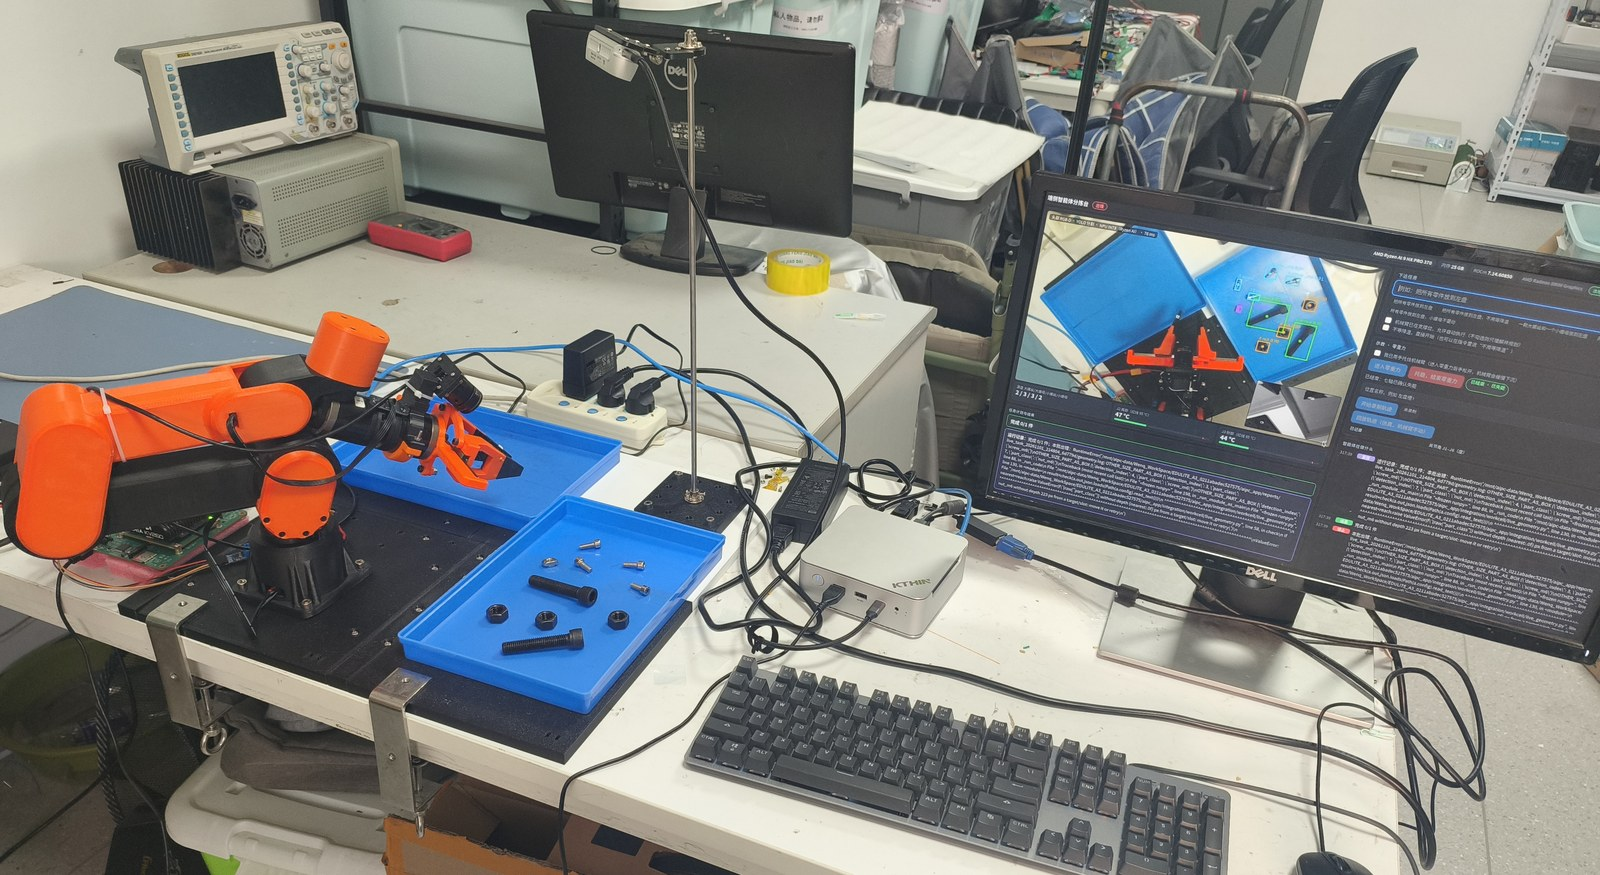
\includegraphics[width=.95\linewidth]{system_overview.jpg}
  \caption{作品全景（斜 45°）：机械臂、左右托盘、头部相机、AI PC 与上位机控制台}\label{fig:overview}
\end{figure}

\subsection{应用领域}

作品以装配配料、维修备件整理中的紧固件分拣为应用背景。用户通过中文指令调整分拣类别和数量，例如从混合零件中挑出小螺母，或将指定数量的螺丝补到目标盘。这种交互方式适合小批量、多任务的桌面工位。

系统采用本地推理，感知、规划和执行模块可分别扩展，也适合作为具身智能、嵌入式控制与 FPGA 教学实验平台。新增零件时可补充训练样本和抓取参数；调整工位时可利用拖动示教记录，为点位配置提供参考。

\subsection{主要技术特点}

\begin{enumerate}
  \item \textbf{NPU 与 GPU 分工}：NPU 运行常驻零件分割，GPU 运行本地大模型，减轻持续检测与大模型生成之间的计算资源竞争。
  \item \textbf{PL 承担周期执行}：已提交的轨迹由 PL 按 5\ms 周期求值并调度 CAN 发送，控制节拍由硬件计数器和截止期队列维持。
  \item \textbf{板端完成局部纠偏}：连续对准在 KV260 内计算视觉修正量，PL 限制关节偏移及其变化速度，减少控制数据的跨机往返。
  \item \textbf{任务与版本关联}：作业包通过内容摘要标识，执行前核对文件、任务和视觉回复的一致性，运行后保留执行及核验记录。
\end{enumerate}

\subsection{主要性能指标}

\begin{table}[H]
  \centering\small
  \caption{主要性能指标（测量条件与证据文件见第三部分与 \texttt{metrics/metrics.csv}）}\label{tab:kpi}
  \begin{tabularx}{\linewidth}{@{}>{\raggedright\arraybackslash}p{4.6cm} Y@{}}
    \toprule
    指标 & 实测值 \\
    \midrule
    零件分割精度 & 掩码 mAP50 0.976，mAP50-95 0.729（四类，验证 imgsz=1280） \\
    检测延迟（单帧，含全分辨率掩码） & GPU P50 45.4\ms；NPU P50 72.1\ms \\
    大模型同载下检测 P95 & NPU 120→141\ms；GPU 67→306\ms \\
    5\ms 周期间隔偏差 & P50 0.4\us，P95 67.0\us（15364 个周期，逻辑分析仪） \\
    PL 掩码核 / ARM 单核 & 7.82 / 14.43\ms，每帧 CPU 耗时降低 95\% \\
    板端对准收敛（大螺丝） & P50 1.06\,s（12/12 次收敛） \\
    视觉到修正指令延迟 & P50 123.0\ms，P95 206.0\ms（407 帧） \\
    跟踪看门狗检测延迟 & PL 300.8\ms；ARM 采样判据 408.1\ms \\
    FPGA 时序 & 100\,MHz，WNS +0.150\,ns，TNS 0.000\,ns \\
    AI PC $\leftrightarrow$ KV260 & RTT P50 0.169\ms，丢包 0.0\% \\
    开发记录中的放置确认比例 & 83/104（79.8\%，数量统计完整的记录），头部相机逐槽核对 \\
    \bottomrule
  \end{tabularx}
\end{table}

\subsection{主要创新点}

\begin{enumerate}
  \item \textbf{面向并发任务的端侧 AI 分工}：将 NPU 常驻分割与 GPU 大模型推理分开部署，用同载测试验证检测尾延迟的改善。
  \item \textbf{视觉与执行在板端衔接}：腕部连续纠偏在 KV260 内完成，由 PL 通道约束修正幅度和速度，缩短局部反馈路径。
  \item \textbf{周期控制与保护一体实现}：PL 集成轨迹求值、CAN 调度、执行保护和图像预处理，以总线实测和软硬件对照验证效果。
\end{enumerate}

\subsection{设计流程}

项目先完成 CAN 通信与轨迹执行，再建立头部识别、空间标定和抓取规划，随后接入腕部纠偏、中文任务接口与结果核验（图~\ref{fig:flow}）。各阶段通过仿真、板端测试和实物运行检查，结合逻辑分析仪、功率读数及任务日志评估表现。大模型工具辅助编码、测试与故障分析，协作记录见附录~\ref{app:collab}。

\begin{figure}[H]
\centering
\begin{tikzpicture}[
  node distance=4mm and 3mm,
  st/.style={draw=blue!60!black,fill=blue!6,rounded corners=2pt,align=center,font=\footnotesize,minimum height=10mm,text width=25mm},
  ar/.style={-{Stealth[length=2mm]},thick,blue!50!black}]
  \node[st] (a) {需求分析\\评分项拆解};
  \node[st,right=of a] (b) {执行层\\CAN · 轨迹 · 守护};
  \node[st,right=of b] (c) {感知层\\采集 · 训练 · 量化};
  \node[st,right=of c] (d) {两端协同\\作业包 · 板端闭环};
  \node[st,below=of d] (e) {实测迭代\\逻辑分析仪 · 功率};
  \node[st,left=of e] (f) {功能扩展\\纠偏 · 复审 · 示教};
  \node[st,left=of f] (g) {归档与复用\\技能包 · 文档};
  \draw[ar] (a)--(b); \draw[ar] (b)--(c); \draw[ar] (c)--(d); \draw[ar] (d)--(e); \draw[ar] (e)--(f); \draw[ar] (f)--(g);
  \begin{scope}[on background layer]
    \node[draw=orange!70!black,fill=orange!8,rounded corners=2pt,fit=(a)(d)(e)(g),inner sep=2.5mm] (llm) {};
  \end{scope}
\end{tikzpicture}
\caption{设计流程}\label{fig:flow}
\end{figure}

\section{系统组成及功能说明}

\subsection{整体介绍}

系统由 AI PC、KV260 和机械臂组成，分工见图~\ref{fig:arch}。AI PC 的 NPU 处理头部相机图像，GPU 运行本地大模型，CPU 进行坐标变换、逆运动学求解与轨迹检查。KV260 的 ARM 处理器（PS）管理作业并运行腕部定位，PL 按 5\ms 周期求值轨迹、调度 CAN 发送，同时执行保护和受限修正。六轴机械臂与夹爪共七个电机接收设定，完成抓取和放置。\doccite{ref:kv260}

头部相机覆盖两个托盘，提供接近目标所需的全局位置；腕部相机在抓取前测量局部偏差。作业包经千兆网线下发到 KV260，连续对准在板内完成。放置结束后，头部相机再次观察目标盘，核对实际结果是否满足任务要求。

\begin{figure}[H]
\centering
\resizebox{\linewidth}{!}{%
\begin{tikzpicture}[
  font=\footnotesize,
  blk/.style={draw=#1!60!black,fill=#1!7,rounded corners=2pt,align=center,minimum height=9mm,text width=27mm},
  blk/.default=blue,
  wide/.style={draw=#1!60!black,fill=#1!7,rounded corners=2pt,align=center,minimum height=9mm,text width=61mm},
  grp/.style={draw=#1!70!black,rounded corners=4pt,inner sep=3mm,thick},
  ar/.style={-{Stealth[length=1.8mm]},semithick},
  lab/.style={font=\scriptsize,inner sep=1.5pt}]
  % AI PC: two input columns feeding one planner
  \node[blk=teal] (cmd) at (0,0) {中文指令};
  \node[blk=teal] (cam) at (34mm,0) {头部相机 D435i\\USB3};
  \node[blk=teal] (llm) at (0,-15mm) {指令理解\\Qwen2.5-VL · \textbf{GPU}};
  \node[blk=teal] (det) at (34mm,-15mm) {零件分割 YOLO11n-seg\\\textbf{NPU} · A8W8};
  \node[wide=teal] (plan) at (17mm,-31mm) {CPU 规划与轨迹检查\\逆运动学 · 轨迹 · MuJoCo};
  \node[wide=teal] (ui) at (17mm,-46mm) {上位机控制台\\核对 · 中文复审 · 示教 · 数字孪生};
  % KV260
  \node[blk=orange] (exe) at (88mm,-31mm) {PS 作业执行\\校验 · 执行链 · 心跳};
  \node[blk=orange] (vl) at (122mm,-31mm) {PS 腕部视觉环\\定位 · 误差 · 修正};
  \node[draw=red!60!black,fill=red!6,rounded corners=2pt,align=center,minimum height=12mm,text width=62mm] (pl) at (105mm,-53mm) {\textbf{PL（100 MHz）}\\5 ms 轨迹求值 · CAN 调度 · 守护 · 看门狗\\图像掩码核 · 在线修正通道};
  % devices
  \node[blk=gray] (wc) at (122mm,-8mm) {腕部相机 OV9281};
  \node[blk=gray,text width=44mm] (arm) at (105mm,-77mm) {EDULite A3 六轴 + 夹爪 · 7 电机};
  \begin{scope}[on background layer]
    \node[grp=teal,fit=(cmd)(cam)(ui),label={[font=\small\bfseries]above:Ryzen AI PC}] {};
    \node[grp=orange,fit=(exe)(vl)(pl),label={[font=\small\bfseries,anchor=south west]north west:Kria KV260}] {};
  \end{scope}
  \draw[ar] (cmd)--(llm); \draw[ar] (cam)--(det);
  \draw[ar] (llm.south)--(llm.south|-plan.north); \draw[ar] (det.south)--(det.south|-plan.north);
  \draw[ar] (plan)--(ui);
  \draw[ar] (plan.east)--node[lab,above,pos=.4]{作业包}node[lab,below,pos=.4]{千兆直连}(exe.west);
  \draw[ar] (wc)--node[lab,right,pos=.25]{USB}(vl);
  \draw[ar] (exe.south)--node[lab,left]{AXI-Lite}(exe.south|-pl.north);
  \draw[ar] (vl.south)--node[lab,right]{修正目标}(vl.south|-pl.north);
  \draw[ar,<->] (pl)--node[lab,right,pos=.72]{CAN 1 Mbps}(arm);
\end{tikzpicture}
}
\caption{系统整体框图}\label{fig:arch}
\end{figure}

一次分拣任务的数据流如下：

\begin{enumerate}
  \item \textbf{理解}：操作员输入中文指令，规则解析或本地大模型生成任务合约（零件类别、数量、目标托盘）。
  \item \textbf{感知}：NPU 对头部相机画面做实例分割，结合深度换算出每个零件在机械臂基座坐标系中的位置与主轴方向。
  \item \textbf{规划}：逆运动学与七次多项式生成关节轨迹，MuJoCo 模型逐段检查碰撞与几何约束，打包成作业包下发。\doccite{ref:trajectory}
  \item \textbf{执行}：KV260 校验作业后把多项式段原子提交给 PL，PL 每 5\ms 求值并经 CAN 发送位置设定。
  \item \textbf{对准}：到达零件上方后，腕部视觉环把像素误差换算为关节偏移写入 PL 修正通道，收敛后下降夹取。
  \item \textbf{核验}：放置完成后回到起点，头部相机逐槽核对，本地大模型对比前后画面给出中文复审。
\end{enumerate}

模型推理与规划放在 AI PC，局部视觉定位放在板端 ARM，定时执行与设定检查放在 PL，具体划分见表~\ref{tab:partition}。

\begin{table}[H]
\centering\small
\caption{软硬件划分依据}\label{tab:partition}
\begin{tabularx}{\linewidth}{@{}>{\raggedright\arraybackslash}p{4.1cm} >{\raggedright\arraybackslash}p{2.2cm} Y@{}}
\toprule
功能 & 位置 & 依据 \\
\midrule
检测、语言理解、规划、校验 & AI PC & 计算量大、算法迭代快；NPU/GPU 本地推理，CPU 规划 \\
轨迹插补与 5\ms 设定发送 & PL & 节拍由 PL 计数器与截止期队列保证，不受 Linux 调度影响 \\
租约、反馈新鲜度、编码范围守护 & PL & 与发送路径同一时钟域，按故障类型限制后续发送 \\
七轴跟踪看门狗 & PL & 逐反馈帧判定七轴，不增加总线负载 \\
腕部图像掩码 & PL & 大螺丝路径的掩码处理 P50 7.82\ms，减少 CPU 耗时 \\
在线修正 & PS 与 PL & PS 只写目标，PL 逐拍限幅限速，对准环不经网络 \\
\bottomrule
\end{tabularx}
\end{table}

\subsection{硬件系统介绍}

\subsubsection{硬件整体介绍}

\begin{table}[H]
\centering\small
\caption{硬件组成}\label{tab:bom}
\begin{tabularx}{\linewidth}{@{}>{\raggedright\arraybackslash}p{1.8cm} >{\raggedright\arraybackslash}p{4.6cm} Y@{}}
\toprule
类别 & 器件 & 主要功能与连接 \\
\midrule
计算主机 & AMD Ryzen AI 9 HX PRO 370 & XDNA2 NPU 分割零件；Radeon 890M 运行大模型；CPU 规划轨迹 \\
控制板 & Kria KV260（K26 SOM） & ARM 管理作业与视觉定位；PL 定时控制、执行保护及掩码加速 \\
执行机构 & EDULite A3 六轴机械臂与夹爪 & 六个关节电机定位末端，夹爪电机完成开合；CAN 1\,Mbps \\
总线接口 & SN65HVD230（3.3\,V） & 连接 PL 逻辑电平与 CAN 差分总线；两端 120\,$\Omega$ 终端 \\
头部相机 & Intel RealSense D435i & USB3 接 AI PC，采集彩色图像与深度，覆盖两个托盘 \\
腕部相机 & OV9281 全局快门 USB 相机 & 固定于夹爪本体，直连 KV260，输出 640×400 灰度图供局部对准 \\
工作台 & 左右两个托盘 & 右盘记为 A，左盘记为 B；B 盘配置 5 个放置槽位 \\

\bottomrule
\end{tabularx}
\end{table}

KV260 与 CAN 收发器经 PMOD J2 连接：J2-1 为 \texttt{can\_tx}（H12，LVCMOS33），J2-3 为 \texttt{can\_rx}（E10），J2-9 为地，J2-11 为 3.3\,V 供电。机械臂独立供电，与 KV260 通过 CAN 差分线和信号地相连。\doccite{ref:can}\doccite{ref:transceiver}

\subsubsection{机械设计介绍}

工位由机械臂、两个托盘和相机支架组成。头部 D435i 固定在托盘上方，同时覆盖两个托盘；腕部相机固定在夹爪的不动本体上，开合时支架不随爪指移动，镜头对焦于抓取对准距离。机械臂 URDF 模型用于正运动学计算、MuJoCo 轨迹检查及数字孪生显示，头部相机及立柱作为静态障碍物参与规划。\doccite{ref:realsense}\doccite{ref:mujoco}\doccite{ref:robotics}

\begin{figure}[H]
  \centering
  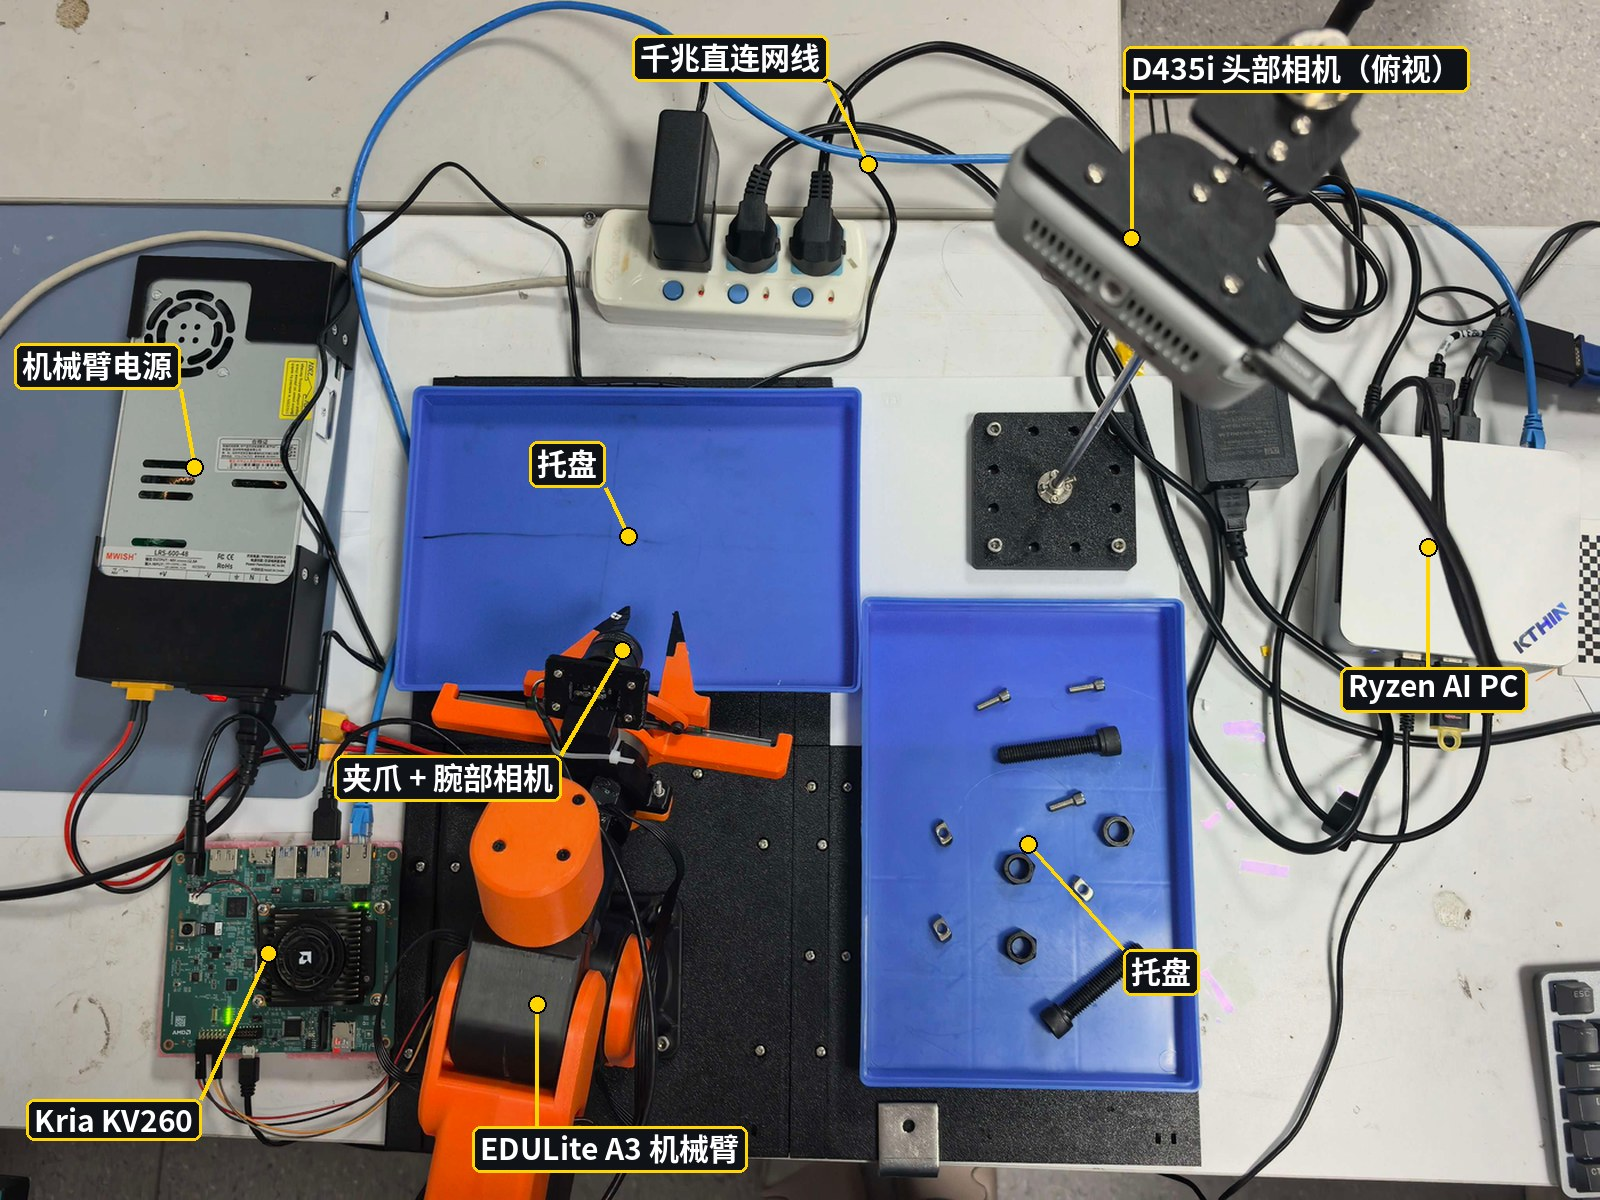
\includegraphics[width=.9\linewidth]{workcell_layout.jpg}
  \caption{工位布局（俯视）}\label{fig:mech}
\end{figure}

\begin{figure}[H]
  \centering
  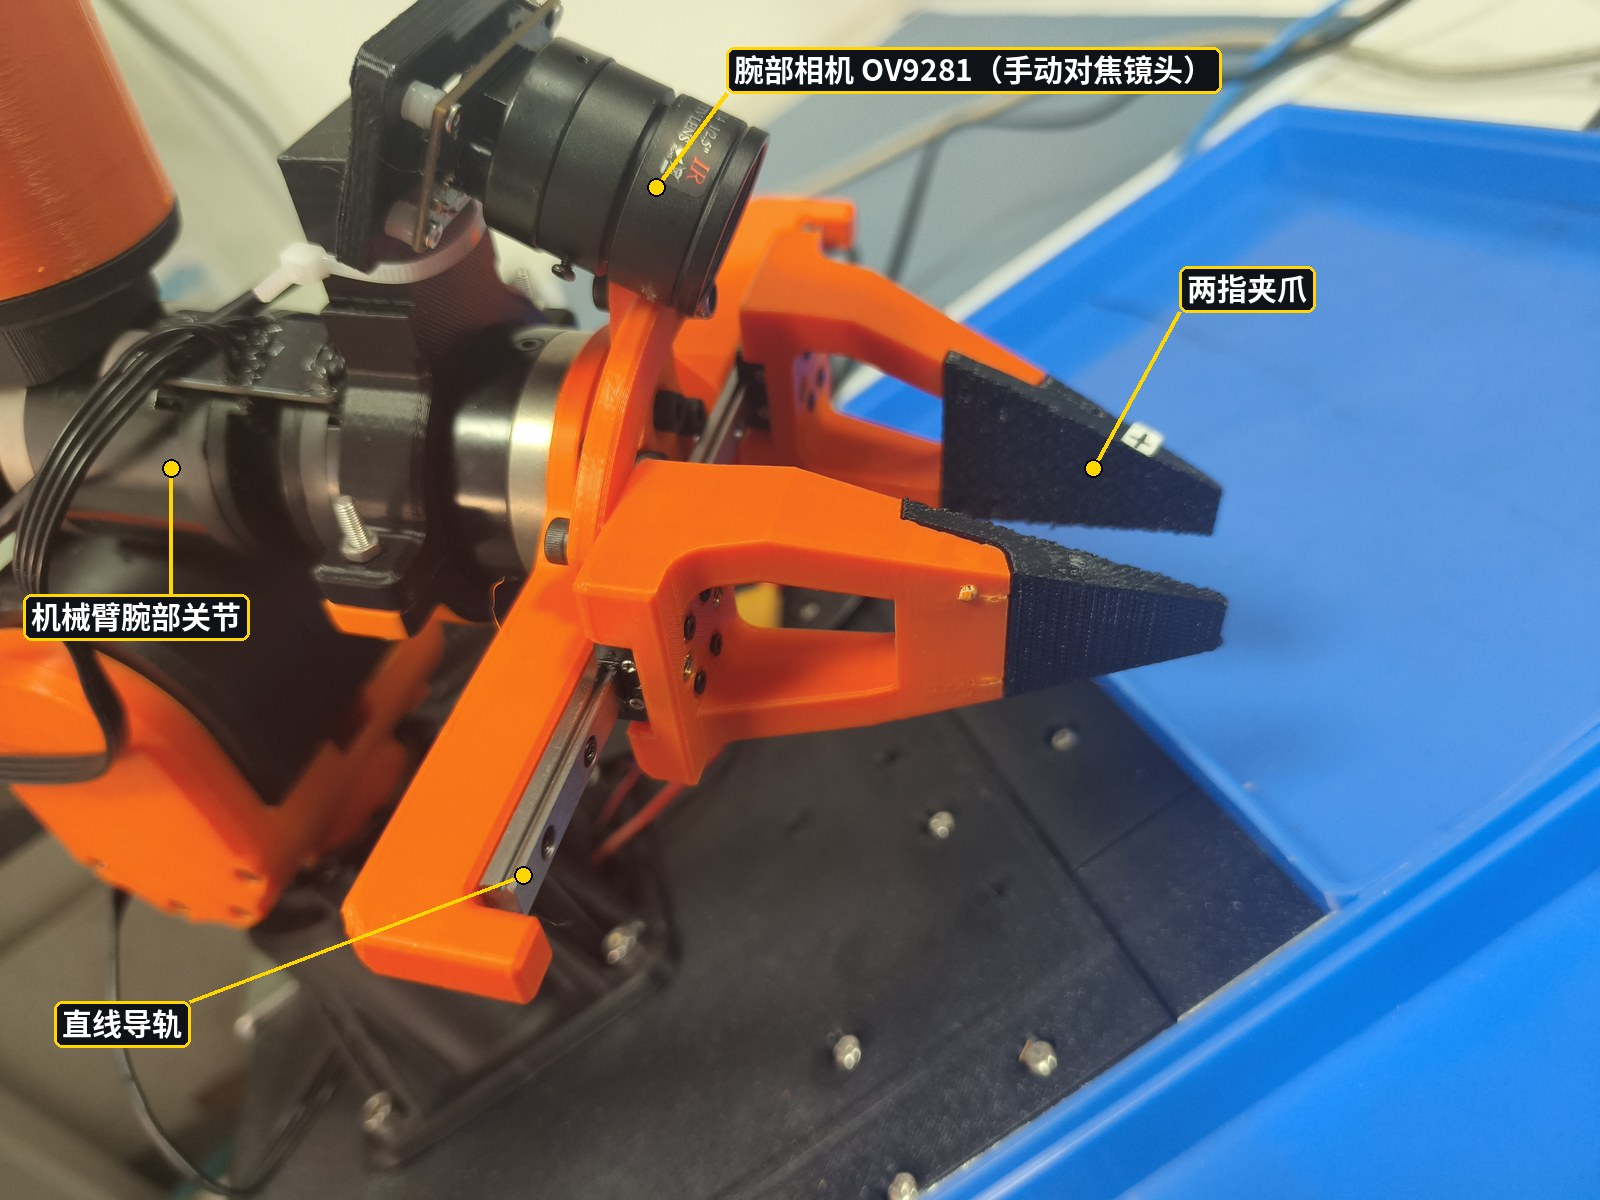
\includegraphics[width=.62\linewidth]{gripper_wrist_camera.jpg}
  \caption{两指夹爪与腕部相机}\label{fig:gripper}
\end{figure}

\subsubsection{电路各模块介绍（KV260 PL 设计）}

PL 内的控制与加速模块运行在 100\,MHz 时钟域，经 AXI-Lite（UIO 窗口）与 PS 交互，视觉核另有 \texttt{m\_axi} 主口直接读帧写掩码（图~\ref{fig:pl}，表~\ref{tab:pl}）。

\begin{figure}[H]
\centering
\resizebox{\linewidth}{!}{%
\begin{tikzpicture}[
  font=\footnotesize,
  m/.style={draw=red!60!black,fill=red!6,rounded corners=2pt,align=center,minimum height=10mm,text width=33mm},
  ps/.style={draw=orange!60!black,fill=orange!8,rounded corners=2pt,align=center,minimum height=10mm,text width=22mm},
  ex/.style={draw=gray!70,fill=gray!10,rounded corners=2pt,align=center,minimum height=10mm,text width=22mm},
  ar/.style={-{Stealth[length=1.6mm]},semithick},
  lab/.style={font=\scriptsize,inner sep=1.5pt}]
  \node[ps] (a53) at (-3mm,0) {PS · A53\\作业执行 · 视觉环};
  \node[ps] (ddr) at (-3mm,-36mm) {DDR\\腕部帧 · 掩码};
  \node[m] (ts) at (44mm,0) {\textsf{trajectory\_stream}\\HLS 七次多项式求值\\在线修正通道};
  \node[m] (ce) at (44mm,-18mm) {\textsf{can\_engine}\\调度 · 租约 · 新鲜度守护};
  \node[m] (vp) at (44mm,-36mm) {HLS \textsf{vision\_pre}\\填充 · 高斯 · Otsu · 闭运算};
  \node[m,text width=24mm] (cc) at (82mm,-18mm) {CAN 位级控制器};
  \node[m,text width=24mm] (tm) at (82mm,0) {\textsf{tracking\_}\allowbreak\textsf{monitor}\\七轴看门狗};
  \node[ex] (tr) at (118mm,-18mm) {SN65HVD230\\7 个电机};
  \begin{scope}[on background layer]
    \node[draw=red!70!black,thick,rounded corners=4pt,fit=(ts)(vp)(cc)(tm),inner sep=3mm,label={[font=\small\bfseries]above:PL（100 MHz 单时钟域）}] {};
  \end{scope}
  \draw[ar,<->] (a53)--node[lab,above]{AXI-Lite}node[lab,below]{UIO 寄存器}(ts);
  \draw[ar] (ts)--node[lab,right]{每 5 ms 设定}(ce);
  \draw[ar] (ce)--(cc);
  \draw[ar,<->] (cc)--node[lab,above]{CAN}node[lab,below]{1 Mbps}(tr);
  \draw[ar] (cc)--node[lab,right]{旁听收发帧}(tm);
  \draw[ar,<->] (ddr)--node[lab,above]{m\_axi}node[lab,below]{DMA}(vp);
  \draw[ar] (a53)--node[lab,left]{写入帧}(ddr);
\end{tikzpicture}
}
\caption{KV260 PL 模块结构}\label{fig:pl}
\end{figure}

\begin{table}[H]
\centering\small
\caption{PL 模块功能与实测}\label{tab:pl}
\begin{tabularx}{\linewidth}{@{}>{\raggedright\arraybackslash}p{3.3cm} Y Y@{}}
\toprule
模块 & 功能 & 实测 \\
\midrule
\path{trajectory_stream} + HLS \texttt{trajectory\_eval} & 每 5\ms 求值七次多项式（Q8.24），生成 Type18 位置设定；截止期队列；原子提交多项式段 & 线上周期偏差 P50 0.4\us；控制服务暂停时最长命令间隔 PL 5.014\ms，ARM 21.435\ms \\
在线修正通道 & 六关节偏移在求值后叠加；每关节限幅、每拍限速、租约；越界故障 & 179 拍逐拍检查与 16/16 回归通过 \\
\texttt{can\_engine} & CAN 收发、反馈表、租约 100\ms、反馈新鲜度、编码范围守护 & 1\,Mbps，总线占用 26.8\% \\
\path{tracking_monitor} & 被动旁听设定帧与反馈帧，七轴跟踪误差看门狗 & 检测延迟 PL 300.8\ms，ARM 判据 408.1\ms \\
HLS \texttt{vision\_pre} & 手指区填充、11 抽头高斯、ROI 内 Otsu、阈值、7×7 闭运算，DMA 读帧写掩码 & 7.82\ms（ARM 14.43\ms），每帧 CPU 0.68\ms；与 ARM 参考逐位一致 \\
\bottomrule
\end{tabularx}
\end{table}

CAN 位级收发采用开源 freecores CAN 控制器（LGPL，保留版权与修改记录）\doccite{ref:freecores}，调度、守护、轨迹、看门狗、修正通道与视觉核均为本项目设计。完整设计实现后占用 LUT 72038（61.51\%）、FF 70273（30.00\%）、BRAM 7.5（5.21\%）、DSP 415（33.25\%），100\,MHz 下 WNS +0.150\,ns、WHS +0.011\,ns，216852 个时序端点满足约束。\doccite{ref:vivado}

在线修正通道的关键寄存器见表~\ref{tab:reg}。通道对写入值检查范围，相关非法写入被忽略并计数；限幅配置在运行中锁定，避免执行过程中改变约束。

\begin{table}[H]
\centering\small
\caption{在线修正通道寄存器（UIO 窗口 0xA0000000 内）}\label{tab:reg}
\begin{tabularx}{\linewidth}{@{}l l Y@{}}
\toprule
偏移 & 名称 & 说明 \\
\midrule
0x840 & ctrl & bit0 使能，bit1 租约过期（只读） \\
0x848 & step & 每 5\ms 最大变化，上限 0.003\,rad \\
0x84C & lease\_us & 目标租约，上限 500\,000\us \\
0x850–0x864 & targets[6] & 六关节偏移目标（Q8.24 rad），写入即续租 \\
0x870–0x884 & applied[6] & 当前已施加偏移（只读） \\
0x8A0–0x8B4 & limits[6] & 每关节偏移限幅，上限 0.25\,rad，运行中锁定 \\
\bottomrule
\end{tabularx}
\end{table}

\subsection{软件系统介绍}

\subsubsection{软件整体介绍}

软件分为 AI PC 端和 KV260 板端，通过网页控制台统一操作（图~\ref{fig:console}）。AI PC 运行 Ubuntu 24.04，PyTorch（ROCm）用于训练与 GPU 推理，AMD Quark 和 Ryzen AI 的 VitisAI EP 用于量化与 NPU 推理。Qwen2.5-VL-3B 常驻 GPU，MuJoCo 用于轨迹几何检查。板端执行器通过 UIO 访问 PL 寄存器；相机服务与视觉环分配到独立 CPU 核，减少其对运动进程心跳的干扰。\doccite{ref:rocm}\doccite{ref:quark}\doccite{ref:ryzen}\doccite{ref:qwen}

\begin{figure}[H]
  \centering
  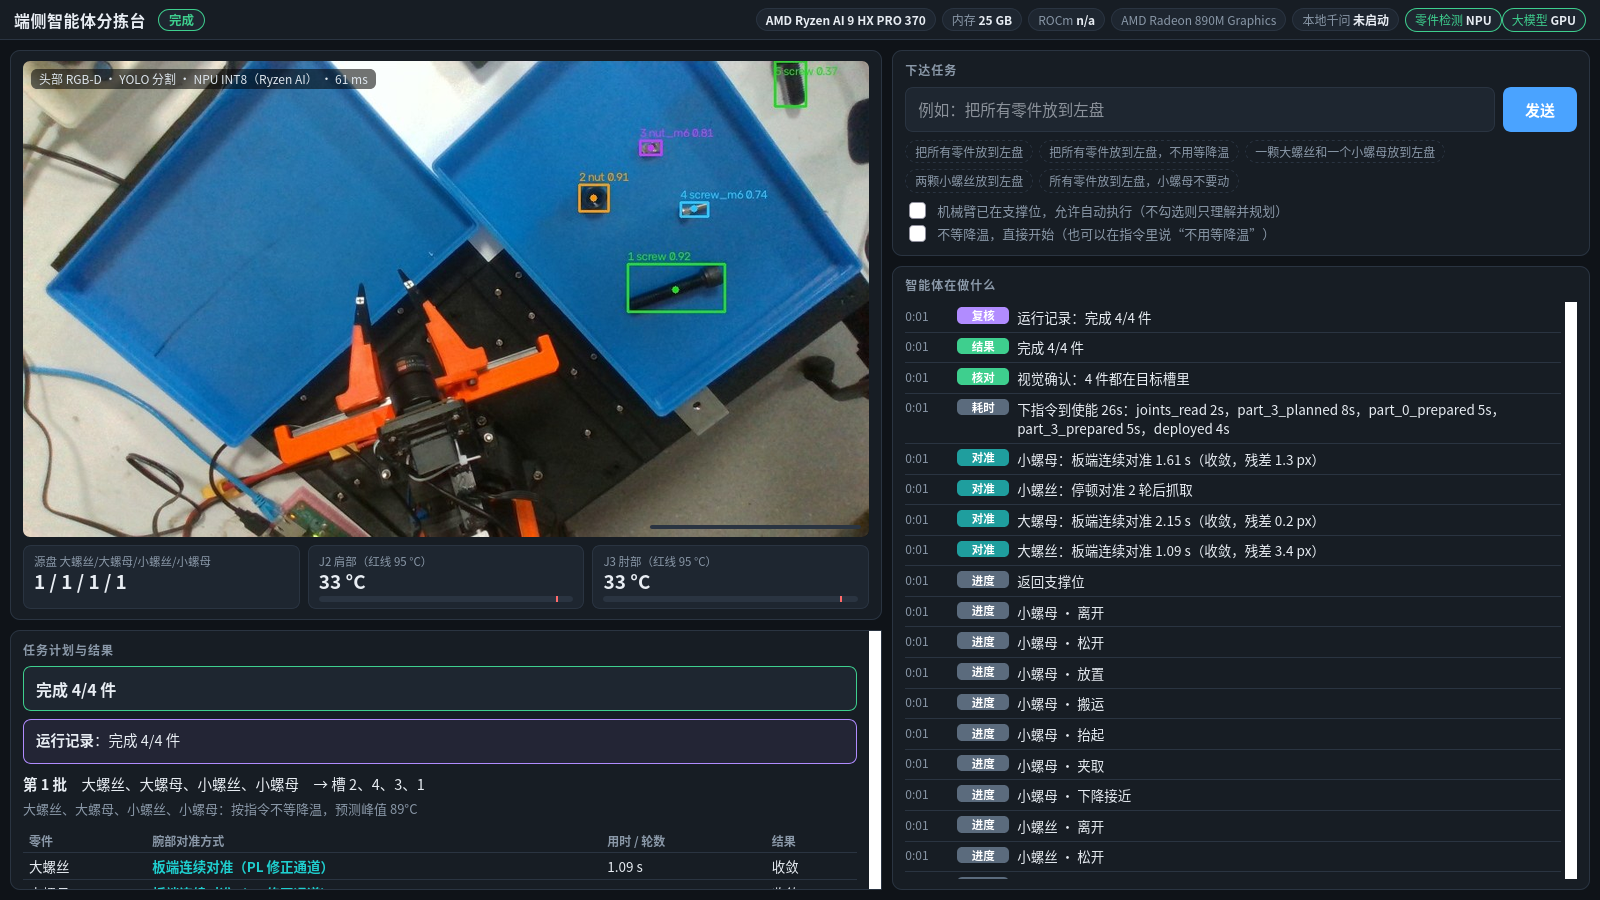
\includegraphics[width=.92\linewidth]{console_four_classes_npu.png}
  \caption{上位机控制台：指令、理解、执行进度、对准方式与复审一屏完成}\label{fig:console}
\end{figure}

\subsubsection{软件各模块介绍}

\begin{figure}[H]
\centering
\begin{tikzpicture}[
  font=\footnotesize,
  s/.style={draw=blue!60!black,fill=blue!6,rounded corners=2pt,align=center,minimum height=8mm,text width=26mm},
  d/.style={draw=orange!70!black,fill=orange!8,diamond,aspect=2.2,align=center,inner sep=1pt,text width=16mm},
  ar/.style={-{Stealth[length=1.6mm]},semithick},
  lab/.style={font=\scriptsize,fill=white,inner sep=1pt}]
  \node[s] (in) {中文指令};
  \node[d,below=4mm of in] (rule) {规则可解析？};
  \node[s,right=6mm of rule] (llm) {本地大模型\\生成候选合约};
  \node[s,below=4mm of rule] (val) {确定性校验\\→ 任务合约};
  \node[s,below=4mm of val] (per) {NPU 分割 + 深度\\→ 零件三维位姿};
  \node[s,below=4mm of per] (pl) {IK · 轨迹生成\\几何检查 · 作业包};
  \node[s,right=46mm of pl] (ex) {KV260 校验\\PL 5 ms 执行};
  \node[s,above=4mm of ex] (al) {腕部对准\\收敛 → 夹取};
  \node[s,above=4mm of al] (pp) {放置 · 返回起点};
  \node[s,above=4mm of pp] (rv) {头部相机核对\\大模型中文复审};
  \draw[ar] (in)--(rule); \draw[ar] (rule)--node[lab,left]{是}(val); \draw[ar] (rule)--node[lab]{否}(llm); \draw[ar] (llm)|-(val);
  \draw[ar] (val)--(per); \draw[ar] (per)--(pl); \draw[ar] (pl)--node[lab]{作业包}(ex);
  \draw[ar] (ex)--(al); \draw[ar] (al)--(pp); \draw[ar] (pp)--(rv);
\end{tikzpicture}
\caption{一次分拣任务的软件流程}\label{fig:swflow}
\end{figure}

\begin{table}[H]
\centering\small
\renewcommand{\arraystretch}{1.08}
\caption{软件模块与关键输入输出}\label{tab:sw}
\begin{tabularx}{\linewidth}{@{}p{2.3cm} Y Y Y@{}}
\toprule
模块 & 输入 & 处理 & 输出 \\
\midrule
指令理解 & 中文句子 & 规则或大模型解析；校验类别、数量和托盘 & 结构化任务 \path{workcell.task.v1} \\
零件感知 & RGB-D 帧 & 实例分割、深度定位、手眼坐标变换 & 基座坐标、主轴、置信度 \\
规划与校验 & 任务、零件位姿 & 逆运动学、轨迹生成、碰撞与速度检查 & 作业包与文件摘要 \\
板端执行 & 作业包 & 摘要校验、段提交、租约续期、事件回报 & PL 命令、执行事件 \\
腕部对准 & 腕部帧、目标点 & 图像定位；像素误差映射为关节偏移 & 修正目标、收敛信号 \\
核对与复审 & 前后画面、日志 & 逐槽计数；大模型对比前后画面 & 核验结果、中文说明 \\
示教与孪生 & 实测关节状态 & 重力补偿、拖动记录、三维渲染 & 关节姿态、轨迹记录 \\
\bottomrule
\end{tabularx}
\end{table}

\paragraph{两端协议。}AI PC 通过 SSH 传输作业包及板端运行文件，以内容摘要标识版本。停顿对准通过 HTTP 交换视觉请求和结果，使用唯一请求标识（nonce）、作业摘要和帧哈希关联当前任务。连续对准通过板内进程通信传递结果，修正计算无需往返 AI PC。

PS 通过 AXI-Lite 读写 PL 寄存器，图像核通过内存主接口读入灰度帧并写回掩码，PL 通过 CAN 29 位扩展帧发送电机设定。各入口分别检查文件一致性、数值范围和运行约束。PL 周期以硬件时钟计时，板端软件延迟以本机时钟计时，统计无需依赖跨机时钟同步。

\paragraph{腕部对准。}系统按零件类别处理腕部图像，提取抓取参考点，计算其与标定对准点之间的像素偏差。图像雅可比将偏差换算为工具平面位移，再映射为关节偏移写入 PL；PL 限制修正幅度和每周期变化量。图~\ref{fig:wrist} 展示图像处理各阶段。\doccite{ref:servo}

大螺丝、大螺母和小螺母采用板端连续对准，小螺丝采用停顿取图对准。大螺丝的手指区填充、高斯滤波、Otsu 阈值和闭运算由 PL 掩码核完成，后续轮廓定位由 PS 完成。连续对准按图像更新偏差，并以 100\,Hz 平滑写入修正目标；连续 3 帧满足阈值后进入下降和夹取。\doccite{ref:otsu}

\begin{figure}[H]
  \centering
  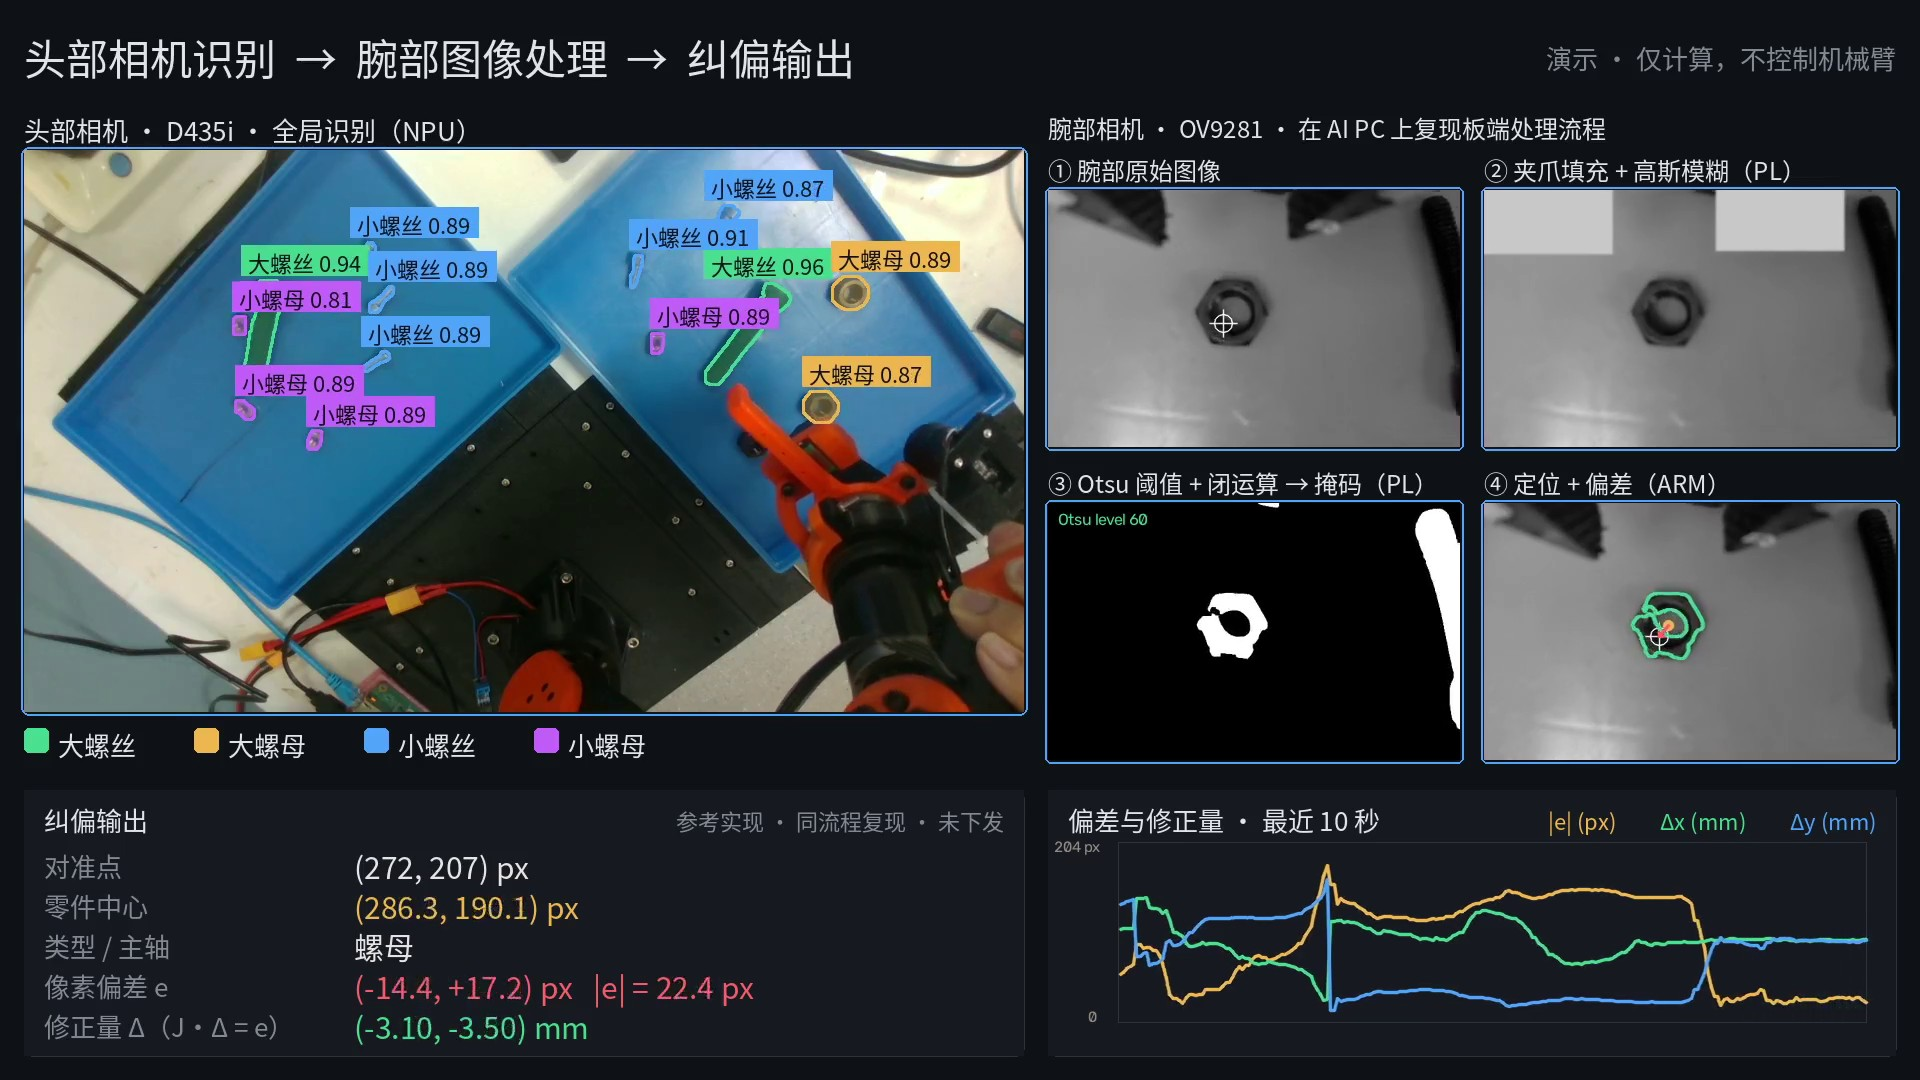
\includegraphics[width=\linewidth]{framework_view.jpg}
  \caption{头部识别与腕部图像处理流程（零重力手拖演示画面，腕部各阶段在 AI PC 上按板端流程复现）}\label{fig:wrist}
\end{figure}

\paragraph{零重力示教与数字孪生。}控制台启动零重力模式后，板端根据实测位姿计算重力补偿力矩，并施加三层力矩上限，辅助操作者手动拖动机械臂。控制台以 50\,ms 间隔读取关节角，通过 URDF 正运动学更新三维模型，并用测得速度补偿显示延迟。用户可记录指定点位的关节姿态或一段拖动轨迹，为点位配置与运动分析提供数据。
\section{完成情况及性能参数}

\subsection{整体介绍}

作品已完成中文指令驱动的零件分拣流程，并提供零重力示教、数字孪生和执行后中文复审。整机部署见图~\ref{fig:overview} 与图~\ref{fig:mech}。本节分别说明工程成果、推理性能、控制时序和任务运行结果；P50 表示中位数，P95 表示第 95 百分位数。


\subsection{工程成果}

\subsubsection{机械成果}

机械臂、夹爪与腕部相机支架构成执行端（图~\ref{fig:gripper}）。相机固定在夹爪本体上，系统通过移动末端，使目标的图像参考点接近标定对准点。头部相机覆盖两个托盘，机械臂与相机立柱模型共同参与轨迹检查；同一机械臂模型用于数字孪生显示。

\subsubsection{电路成果}

KV260 经 PMOD J2 与 SN65HVD230 收发器相连，驱动 1\,Mbps CAN 总线上的 7 个电机；腕部相机 USB 直连 KV260。PL 设计在 Vivado 2025.2 下完成综合与实现：LUT 72038（61.51\%）、DSP 415（33.25\%），100\,MHz 时序收敛（WNS +0.150\,ns，216852 个端点全部满足），所有 RTL 模块均有 xsim 回归，HLS 核均通过 C 仿真与 C/RTL 联合仿真。

\begin{figure}[H]
  \centering
  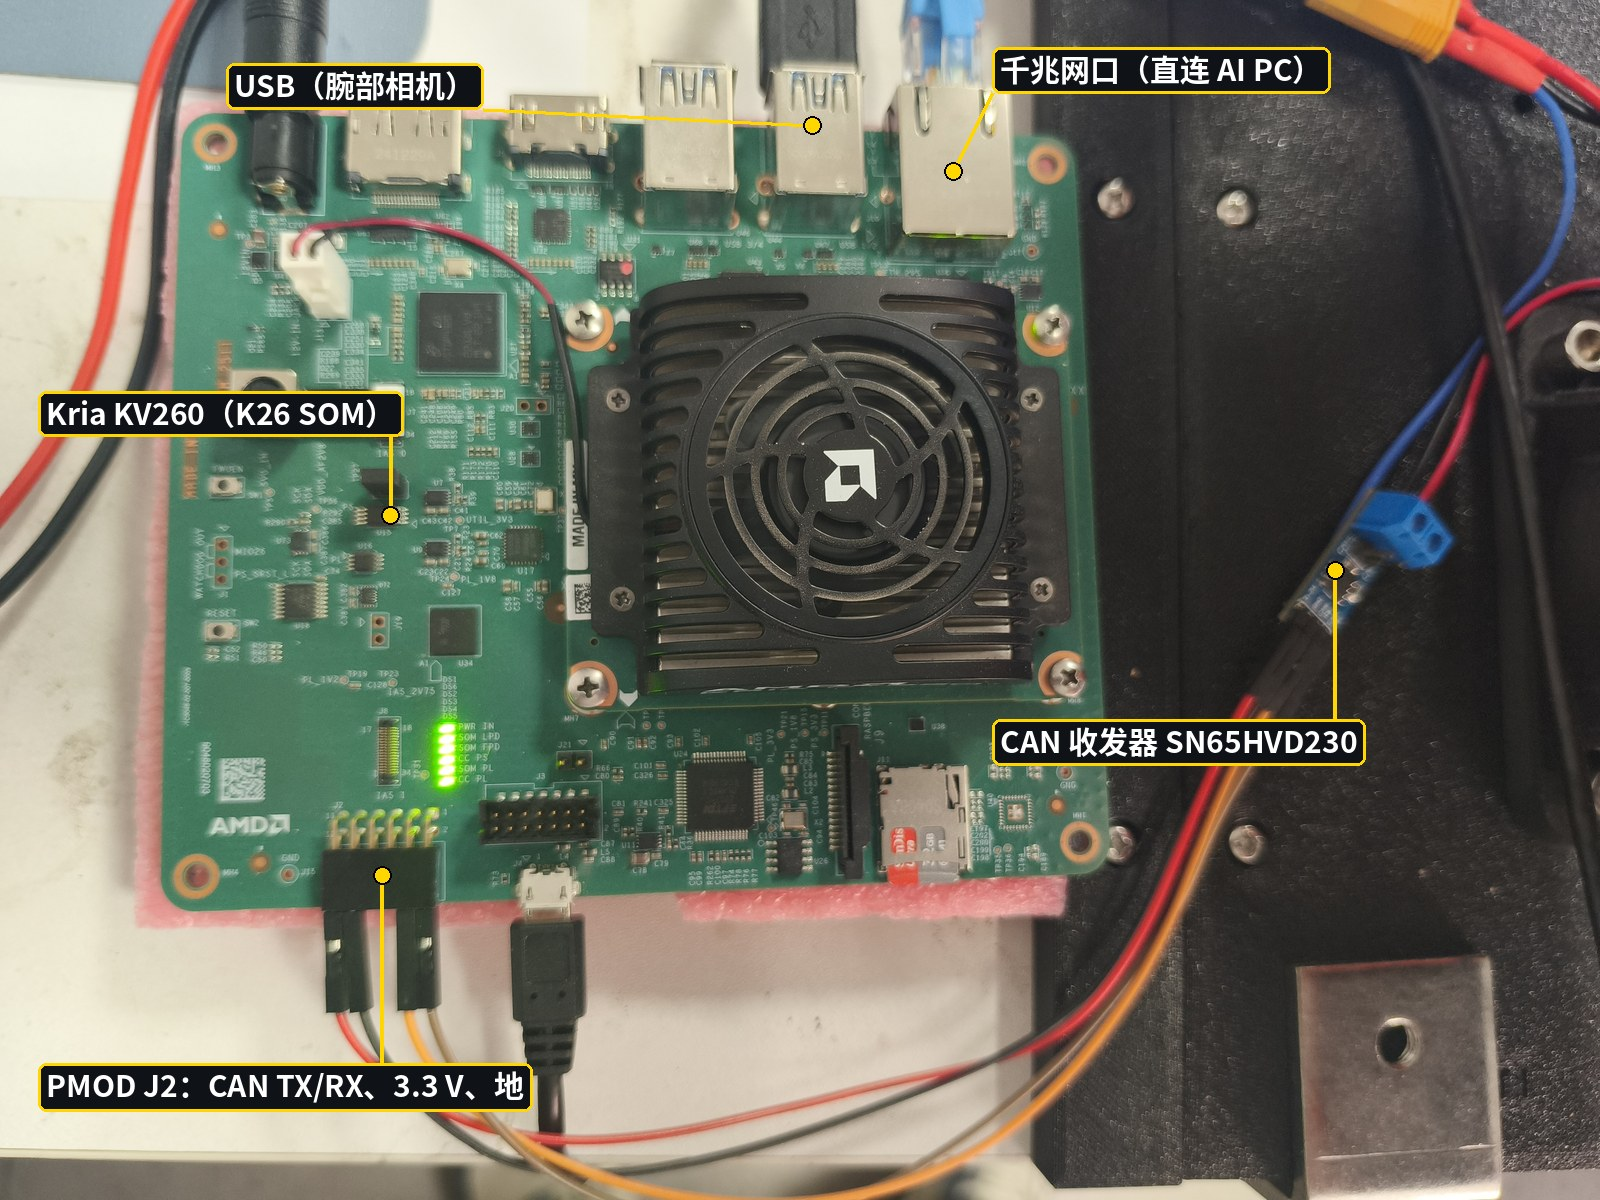
\includegraphics[width=.8\linewidth]{kv260_wiring.jpg}
  \caption{KV260 与 CAN 收发器接线}\label{fig:kv260}
\end{figure}

\subsubsection{软件成果}

上位机控制台集中显示中文指令、解析结果、执行进度、每件零件的对准用时和最终核验结果（图~\ref{fig:console}）。示教区域提供零重力启停、姿态记录和轨迹录制，数字孪生按实测关节角更新。板端软件按内容摘要发布，已有版本可复用，启动时校验源文件摘要，使作业与运行版本对应。

\subsection{特性成果}

\subsubsection{零件识别精度与端侧推理}

四类实例分割模型 YOLO11n-seg 在 AI PC 上用 ROCm 训练，验证集掩码 mAP50 为 0.976、mAP50-95 为 0.729，框 mAP50-95 为 0.852。量化后，用 80 帧图像对照 NPU 与 GPU 后端的抓取目标输出：匹配 270 个三维目标，可抓判定 270/270 一致，两后端输出的基座坐标差值 P50 为 0.33\,mm。\doccite{ref:yolo}

检测延迟见表~\ref{tab:det}。相机采集 1920×1080 图像，经缩放、填充后形成 736×1280 网络输入。后处理还原全分辨率掩码；验证使用 imgsz=1280。

\begin{table}[H]
\centering\small
\caption{头部检测单帧延迟（batch=1，1920×1080 原图，含全分辨率掩码，100 次）}\label{tab:det}
\begin{tabularx}{\linewidth}{@{}l C C C C@{}}
\toprule
后端 & 预处理 P50 & 推理 P50 & 后处理 P50 & 总延迟 P50 / P95 \\
\midrule
GPU（ROCm，FP32） & 8.7\ms & 29.8\ms & 4.6\ms & 45.4 / 49.1\ms \\
NPU（Quark A8W8） & 16.9\ms & 51.9\ms & 2.5\ms & 72.1 / 109.4\ms \\
\bottomrule
\end{tabularx}
\end{table}

\subsubsection{NPU/GPU 异构同载}

单独运行检测时，GPU 延迟较低；与大模型同时运行后，GPU 检测 P95 由 67\ms 升至 306\ms，NPU 检测 P95 由 120\ms 增至 141\ms（图~\ref{fig:contention}）。因此，系统将需要持续运行的分割任务部署到 NPU，把 GPU 留给大模型，以减轻并发推理对检测尾延迟的影响。

\begin{figure}[H]
  \centering
  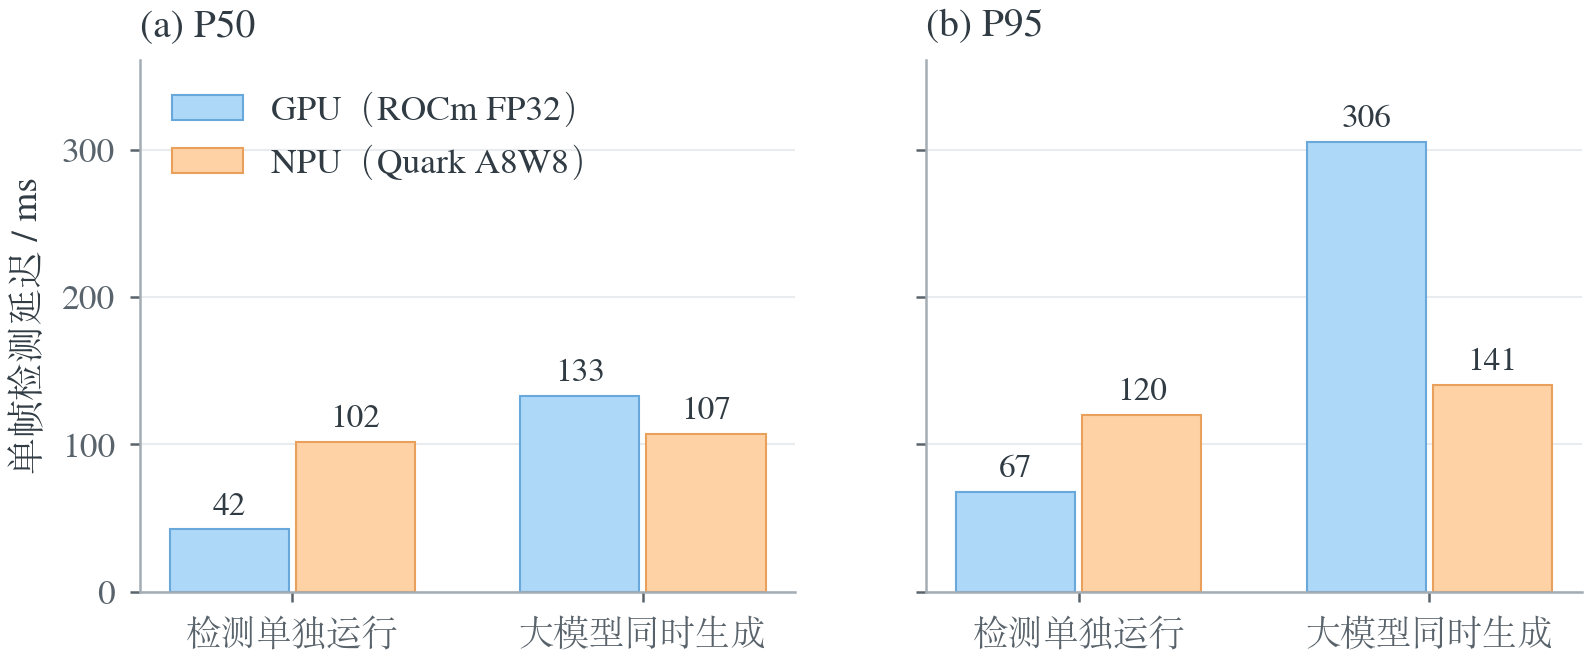
\includegraphics[width=\linewidth]{doc_contention.png}
  \caption{检测单独运行与大模型同时生成时的单帧检测延迟（每档 60 次）}\label{fig:contention}
\end{figure}

\subsubsection{5 ms 控制周期的线上实测}

用 Kingst LA2016 逻辑分析仪（50\,MHz 采样）在 CAN-H 上直接测量：位宽 1.0\us（1\,Mbps），总线占用 26.8\%。PL 轨迹流稳态段 77\,s、15364 个周期中，指令帧起点间隔 P50 4.9998\ms，周期间隔偏差 P50 0.4\us、P95 67.0\us。偏差按相邻指令帧起点间隔与 5\ms 的绝对差计算；周期锚定绝对时间栅格，图中晚点后的周期恢复到栅格，避免逐周期累积。游标实测相邻两个周期的同一指令帧起点相隔 4.99974\ms（图~\ref{fig:la}）。

\begin{figure}[H]
  \centering
  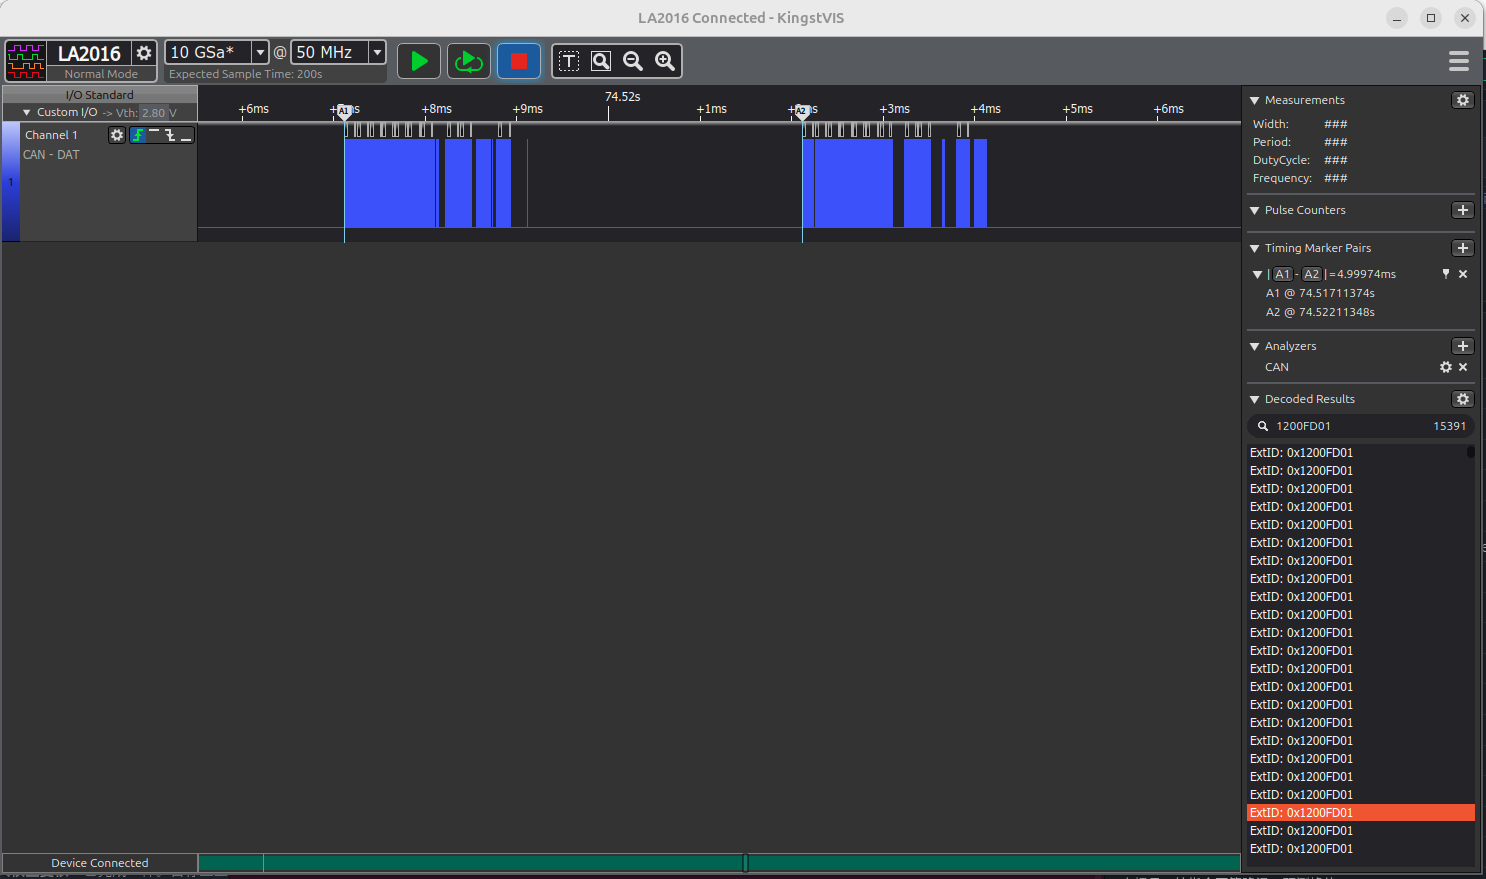
\includegraphics[width=.92\linewidth]{la_marker_5ms.png}
  \caption{逻辑分析仪实测：相邻两个 5 ms 周期的指令帧起点}\label{fig:la}
\end{figure}

\begin{figure}[H]
  \centering
  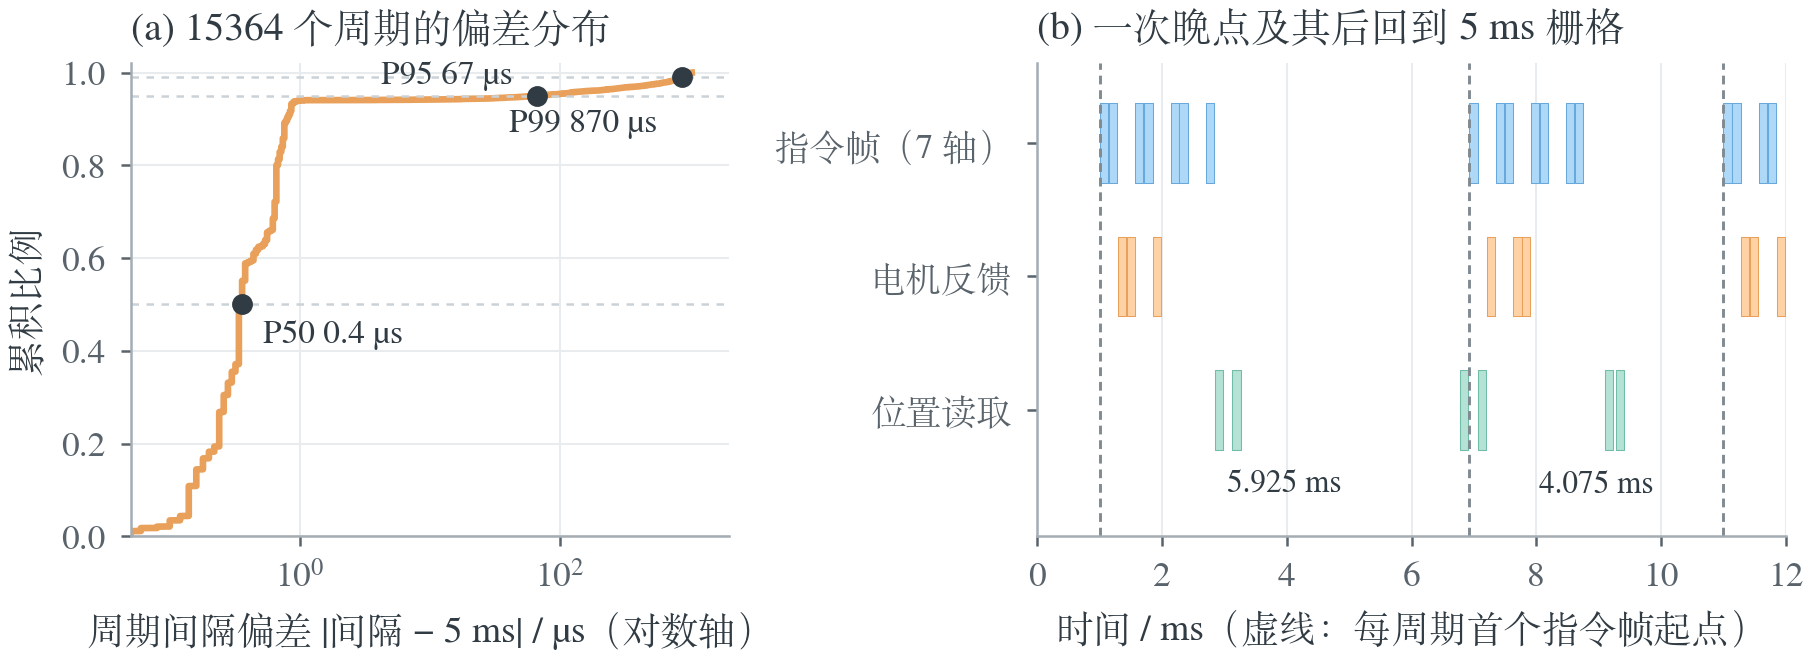
\includegraphics[width=\linewidth]{doc_wire.png}
  \caption{逻辑分析仪实测的 5 ms 周期：(a) 周期间隔偏差的累积分布；(b) 线上帧时序，晚点后下一周期回到栅格}\label{fig:wire}
\end{figure}

\subsubsection{关节跟踪与反馈时序}

一次完整四件运行（132\,s）中，J2 指令对反馈位置跟踪 RMSE 3.4\,mrad，J3 为 5.3\,mrad；七台电机反馈帧间隔（PL 1\us 计数器时间戳，名义 5\ms）P50 5.0\ms、P95 5.047\ms，间隔超过两倍中位数的次数为 0（图~\ref{fig:track}）。

\begin{figure}[H]
  \centering
  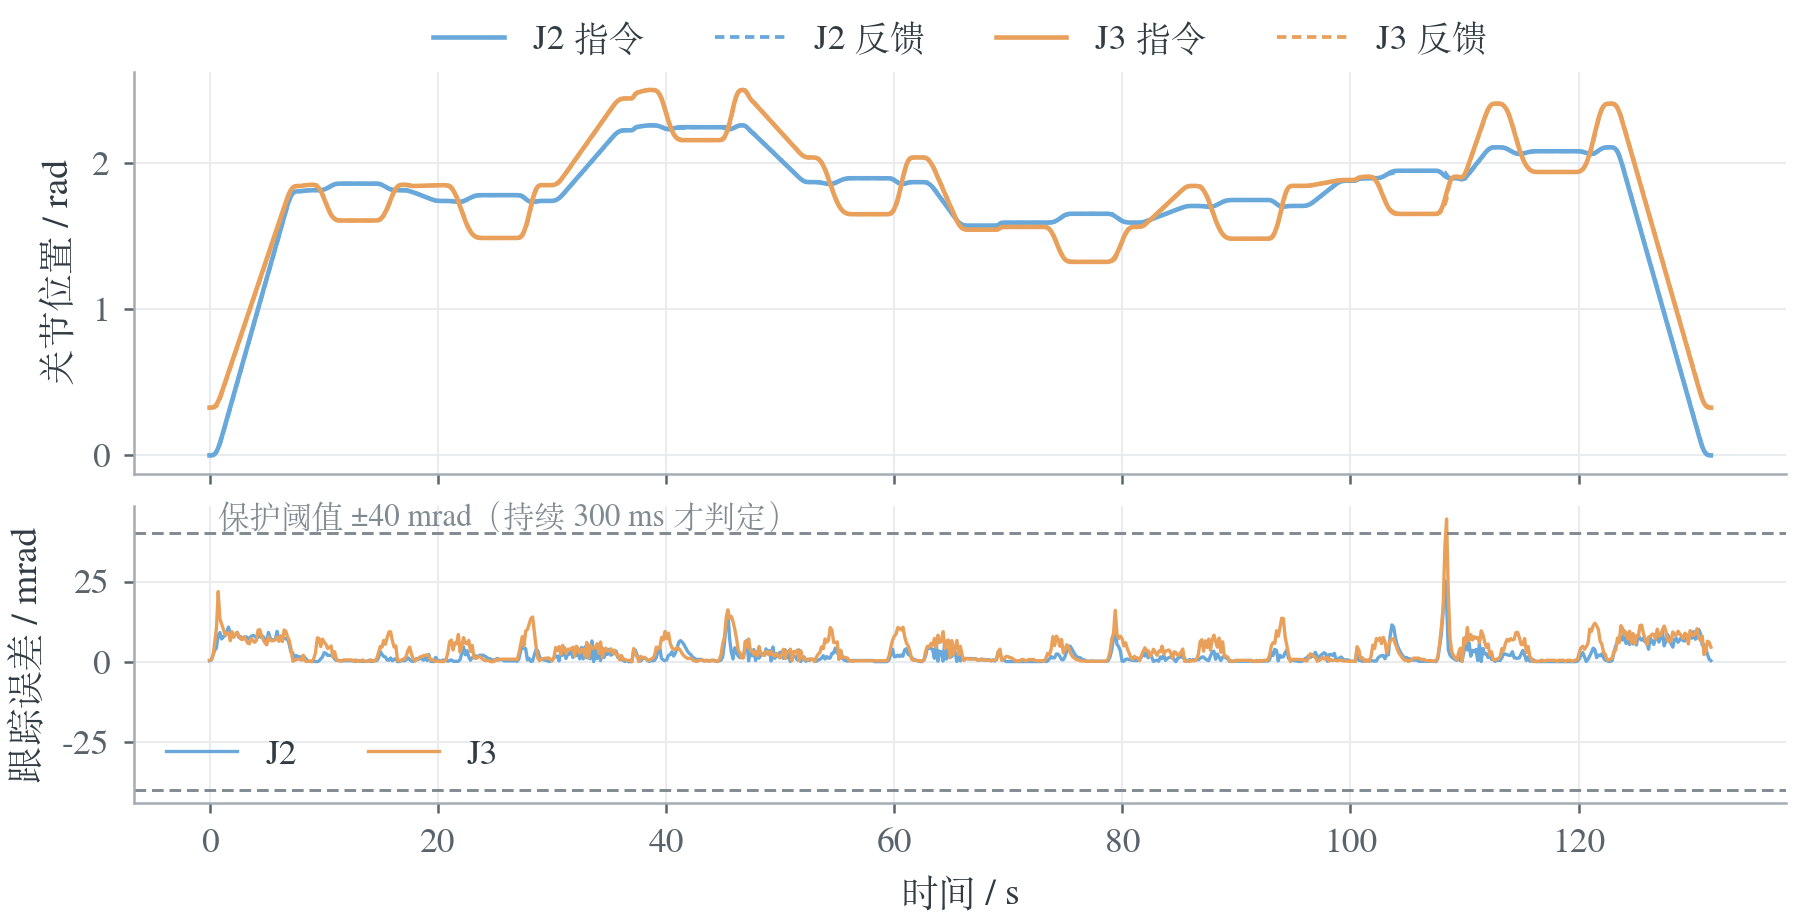
\includegraphics[width=\linewidth]{doc_tracking.png}
  \caption{一次完整四件运行中 J2、J3 的指令与反馈位置（上）及跟踪误差（下）}\label{fig:track}
\end{figure}

\subsubsection{板端闭环对准}

连续对准时，腕部定位与修正计算在 KV260 内完成。407 帧日志中，从腕部帧到达板端到写入 PL 修正目标的延迟 P50 为 123.0\ms、P95 为 206.0\ms，视觉环周期 P50 为 120.0\ms。从悬停到对准收敛，大螺丝用时 P50 为 1.06\,s（12/12 次收敛），大螺母为 2.43\,s（10/11 次收敛），小螺母为 1.61\,s（4/4 次收敛）。

图~\ref{fig:align} 同时列出历史停顿对准的 35 件记录，其悬停到开始下降用时 P50 为 6.67\,s；连续对准统计到收敛，两组计时终点分别标注。采用 CPU 核隔离后的 9 段记录中，各段控制心跳最大间隔的 P50 为 44.5\ms，全部记录的最大间隔为 51.7\ms，低于 PL 的 100\ms 租约。

\begin{figure}[H]
  \centering
  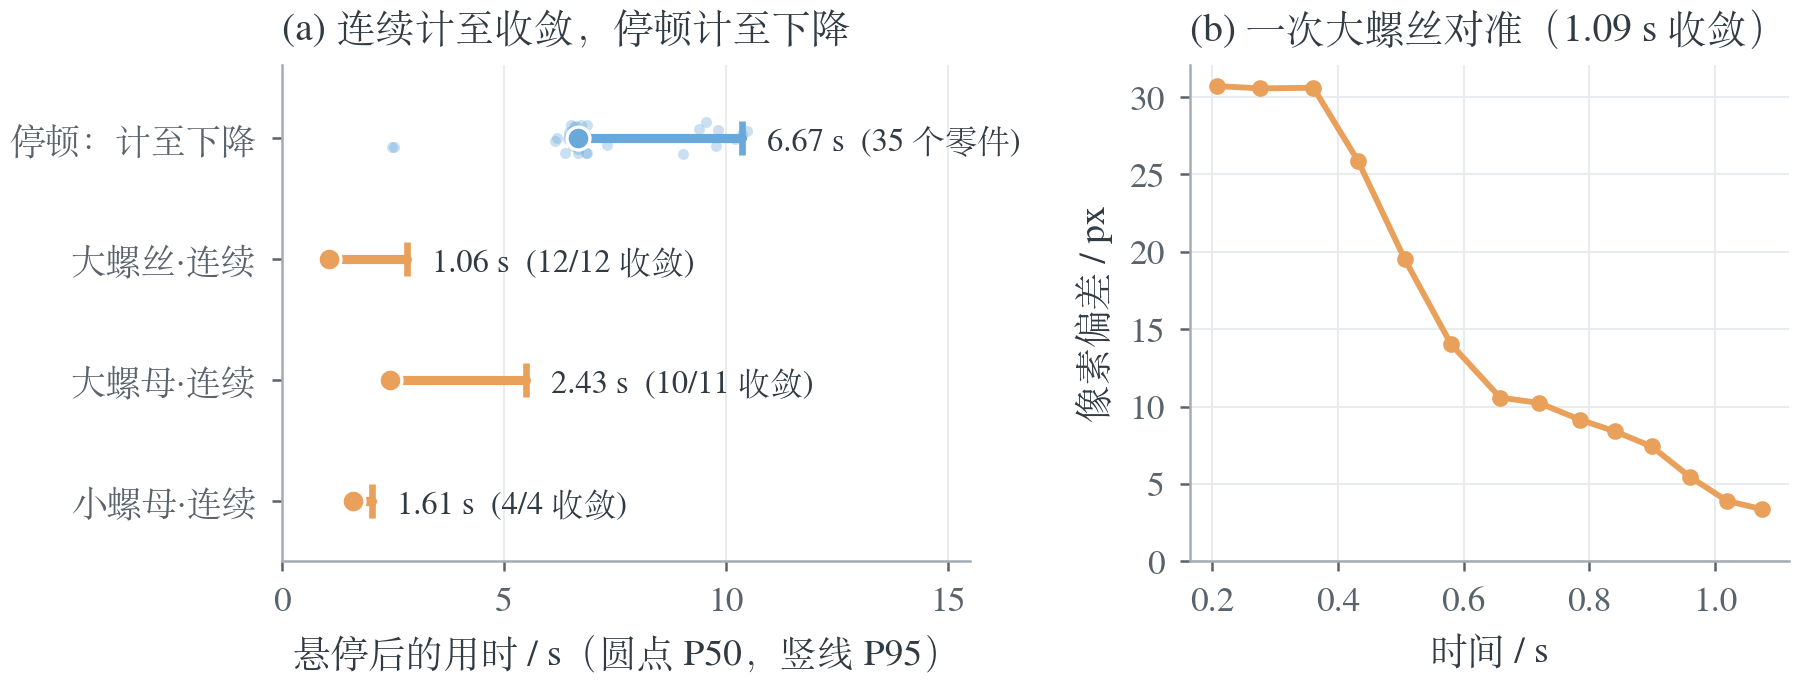
\includegraphics[width=\linewidth]{doc_alignment.png}
  \caption{(a) 连续对准计至收敛，停顿对准计至开始下降（浅色点为逐件数据）；(b) 一次大螺丝对准的像素偏差收敛过程}\label{fig:align}
\end{figure}

\subsubsection{PL 硬件加速与守护}

\begin{figure}[H]
  \centering
  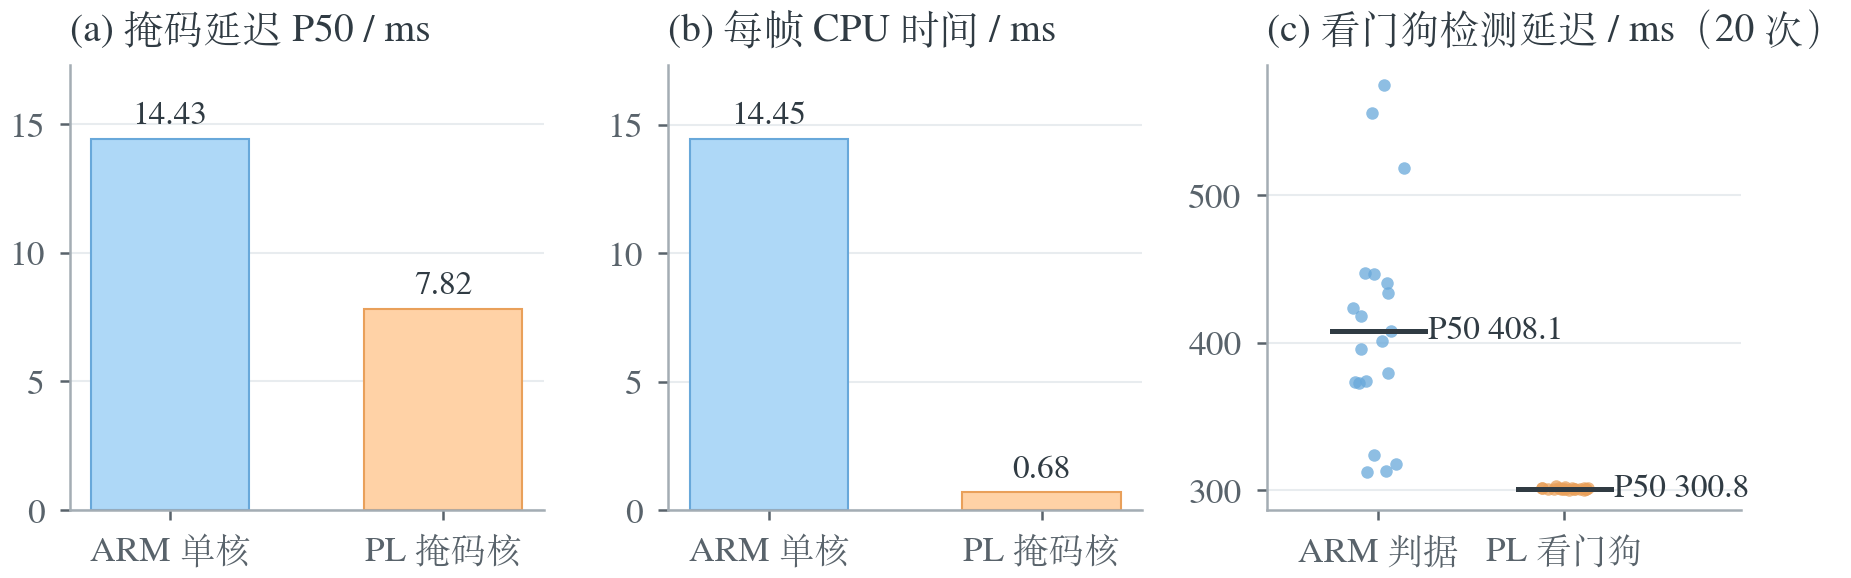
\includegraphics[width=\linewidth]{doc_pl_vs_arm.png}
  \caption{PL 与 ARM 实现对比：(a)(b) 腕部图像掩码，300 帧；(c) 七轴跟踪看门狗，逐次结果与中位数}\label{fig:plarm}
\end{figure}

\begin{table}[H]
\centering\small
\caption{PL 与 ARM 软件实现对比}\label{tab:plarm}
\begin{tabularx}{\linewidth}{@{}>{\raggedright\arraybackslash}p{3.4cm} c c Y@{}}
\toprule
功能 & PL & ARM & 说明 \\
\midrule
腕部图像掩码（P50） & 7.82\ms & 14.43\ms & 300 帧；每帧 CPU 耗时 0.68 对 14.45\ms，降低 95\%；结果逐位一致 \\
控制服务暂停 20\ms 时最长命令间隔 & 5.014\ms & 21.435\ms & 同一参考轨迹 ABBA 对照，PL 维持已提交轨迹的发送节拍 \\
跟踪看门狗检测延迟（P50） & 300.8\ms & 408.1\ms & 20 次板内回环测试；PL 逐帧判定七轴 \\
抓取轨迹 MMIO 写入次数 & \multicolumn{2}{c}{降低 87.59\%} & PL 段提交替代 ARM 逐拍写 \\
\bottomrule
\end{tabularx}
\end{table}

\subsubsection{通信与功耗}

AI PC 与 KV260 千兆直连，200 个 ICMP 包的 RTT P50 为 0.169\ms、P99 为 0.25\ms，测量期间零丢包。作业包通道的有效吞吐为 AI PC 到 KV260 28.2\,MB/s、反向 32.3\,MB/s。

AI PC 的 SoC 功率在空闲、GPU 检测循环和 NPU 检测循环下分别为 23.0\,W、55.6\,W 和 54.3\,W。KV260 测量的是整板功率，空闲为 3.34\,W，A53 单核执行掩码处理时为 3.68\,W。

\subsubsection{任务完成情况}

系统已完成四类零件从指令解析、目标识别到抓取放置、逐槽核对和中文复审的流程，并记录了四件零件在一次会话中全部完成搬运、核对通过的实例。任务接口支持按类别和数量分拣；大螺丝还完成了双向搬运与目标数量调节，可按“多的退回、少的补入”调整目标盘数量。示教与数字孪生提供姿态记录和状态观察。

2026-10-28 至 2026-11-01 的开发记录中，数量统计完整的任务共计划放置 104 件，头部相机确认 83 件，确认比例为 79.8\%。逐次任务、放置核对和运行数据保存在 \path{metrics/logs/task_trials.csv}，典型完整运行的跟踪与对准数据见本节图表。
\section{总结}

\subsection{可扩展之处}

\begin{enumerate}
  \item \textbf{扩展连续视觉对准}：将现有板端连续对准扩展到小螺丝，结合运动中的图像更新，缩短接近与对准之间的等待。
  \item \textbf{扩展零件与工位}：增加垫片、销钉等零件的识别样本和抓取参数，将示教记录接入槽位配置，简化工位调整。
  \item \textbf{进一步利用 PL}：在现有掩码核之后评估轮廓和矩计算的硬件实现，并优化位置读取与 CAN 周期调度的配合。
  \item \textbf{复用工程工具}：将 CAN 时序分析、NPU 部署和工位运维流程整理为通用工具，支持其他 Kria 与 CAN 执行器项目。
\end{enumerate}

\subsection{心得体会}

本项目首先解决的是计算任务的分工。模型推理和轨迹规划适合放在 AI PC，需要接近执行端的腕部定位放在 KV260 的 ARM，周期执行和设定检查交给 PL。最初由 ARM 软件逐拍发送 CAN 设定时，控制服务暂停 20\ms 会使最长命令间隔达到 21.435\ms；改为 PL 执行后，同一对照中的最长间隔为 5.014\ms。随后用逻辑分析仪测量总线，确认硬件周期在真实通信中得到保持。

NPU 部署的价值体现在并发运行。单独检测时 GPU 更快，但大模型同时生成时，GPU 检测尾延迟明显增加。将持续检测放到 NPU 后，系统可以在解析指令、复审结果的同时保持视觉更新。量化中遇到过类别分数因统一 INT8 尺度而失真的问题，最终保留解码节点的浮点计算，再逐点比较两种后端的抓取判定和坐标输出，确认量化模型能够接入原有流程。

腕部纠偏则解决了全局定位与实际夹取之间的偏差。头部相机适合观察整盘目标，腕部相机适合接近目标后的局部测量。将连续对准移到 KV260 内，减少了图像回传和修正下发的等待；修正量由 PL 限幅、限速，再与轨迹求值结果叠加。大螺丝从悬停到收敛的用时 P50 为 1.06\,s，这一过程体现了板端视觉与硬件执行的配合。

实物调试还需要把停止运动与撤掉力矩分开处理。是否回到承托位置、关节反馈是否可信，会影响故障后的处置。因此，我们把异常检测、返回流程和人工介入一起设计，正常回位后结束使能，中途故障则按状态处理。保护条件和处置过程均保留运行记录，便于复查。

大模型工具参与了编码、测试、日志分析和文档整理。有效的协作方式是提供明确任务、接口和原始记录，对生成的修改做回归验证，并用实测检验结论。AMD Ross 的 HLS 技能帮助规范了可综合性检查和构建步骤。部署方法、协作规则及常见故障整理为附录中的技能包，供后续开发复用。

\section{参考文献}

{\small\raggedright
\begin{enumerate}[label={[\arabic*]},ref=\arabic*,leftmargin=2.2em,itemsep=1pt]
  \item\label{ref:kv260} AMD. Kria KV260 Vision AI Starter Kit User Guide (UG1089)[Z]. 2024.
  \item\label{ref:hls} AMD. Vitis High-Level Synthesis User Guide (UG1399)[Z]. 2025.
  \item\label{ref:vivado} AMD. Vivado Design Suite User Guide: Synthesis (UG901) / Implementation (UG904)[Z]. 2025.
  \item\label{ref:ryzen} AMD. Ryzen AI Software Documentation, Release 1.8[EB/OL]. \url{https://ryzenai.docs.amd.com}, 2026.
  \item\label{ref:quark} AMD. Quark Model Quantization Library Documentation[EB/OL]. \url{https://quark.docs.amd.com}, 2026.
  \item\label{ref:rocm} AMD. ROCm Documentation[EB/OL]. \url{https://rocm.docs.amd.com}, 2026.
  \item\label{ref:yolo} JOCHER G, QIU J. Ultralytics YOLO11[CP/OL]. \url{https://github.com/ultralytics/ultralytics}, 2024.
  \item\label{ref:qwen} BAI S, CHEN K, LIU X, et al. Qwen2.5-VL Technical Report[R/OL]. arXiv:2502.13923, 2025.
  \item\label{ref:lora} HU E J, SHEN Y, WALLIS P, et al. LoRA: Low-Rank Adaptation of Large Language Models[C]//\allowbreak International Conference on Learning Representations. 2022.
  \item\label{ref:mujoco} TODOROV E, EREZ T, TASSA Y. MuJoCo: A Physics Engine for Model-Based Control[C]//\allowbreak IEEE/RSJ International Conference on Intelligent Robots and Systems. 2012: 5026-5033.
  \item\label{ref:otsu} OTSU N. A Threshold Selection Method from Gray-Level Histograms[J]. IEEE Transactions on Systems, Man, and Cybernetics, 1979, 9(1): 62-66.
  \item\label{ref:servo} CHAUMETTE F, HUTCHINSON S. Visual Servo Control, Part I: Basic Approaches[J]. IEEE Robotics \& Automation Magazine, 2006, 13(4): 82-90.
  \item\label{ref:trajectory} BIAGIOTTI L, MELCHIORRI C. Trajectory Planning for Automatic Machines and Robots[M]. Berlin: Springer, 2008.
  \item\label{ref:robotics} SICILIANO B, SCIAVICCO L, VILLANI L, et al. Robotics: Modelling, Planning and Control[M]. London: Springer, 2009.
  \item\label{ref:can} ISO 11898-1:2015. Road Vehicles — Controller Area Network (CAN) — Part 1: Data Link Layer and Physical Signalling[S]. 2015.
  \item\label{ref:transceiver} Texas Instruments. SN65HVD23x 3.3-V CAN Bus Transceivers Datasheet[Z]. 2018.
  \item\label{ref:realsense} Intel. Intel RealSense D400 Series Product Family Datasheet[Z]. 2023.
  \item\label{ref:freecores} OpenCores. CAN Protocol Controller (freecores/can)[CP/OL]. \url{https://github.com/freecores/can}.
\end{enumerate}
}

\appendix
\renewcommand{\thesubsection}{\Alph{section}.\arabic{subsection}}
\section{大模型协作记录}\label{app:collab}

\subsection{智能体工作流}

本作品使用大模型工具辅助开发、调试、测试和文档整理，分工如下（图~\ref{fig:agents}）：

\begin{itemize}
  \item \textbf{Claude Code}：参与应用集成、板端视觉、性能分析与提交材料整理；通过代码、日志、测试和仪器数据核对实现。
  \item \textbf{Codex}：参与控制链路开发、故障排查、集成验证与材料审查；结合 AMD Ross 完成七轴插补核的 HLS 检查与构建（附录~C）。
  \item \textbf{交叉评审}：两个智能体结合源代码和实测记录复核改动；离线测试通过后，再在操作员授权范围内验证硬件。
\end{itemize}

\begin{figure}[H]
\centering
\begin{tikzpicture}[font=\footnotesize,
  a/.style={draw=blue!60!black,fill=blue!6,rounded corners=2pt,align=center,minimum height=10mm,text width=32mm},
  h/.style={draw=orange!70!black,fill=orange!8,rounded corners=2pt,align=center,minimum height=10mm,text width=32mm},
  ar/.style={-{Stealth[length=1.6mm]},semithick},lab/.style={font=\scriptsize,inner sep=1.5pt}]
  \node[h] (u) at (0,0) {开发者\\目标 · 规则 · 物理确认};
  \node[a] (c) at (52mm,0) {开发智能体\\编码 · 测试 · 排障 · 文档};
  \node[a] (x) at (52mm,22mm) {Codex + AMD Ross\\HLS 可综合检查与构建};
  \node[a] (g) at (52mm,-22mm) {交叉评审\\代码 · 测试 · 实测记录};
  \node[h] (e) at (104mm,0) {证据\\日志 · 测试 · 仪器数据};
  \node[h] (s) at (104mm,-22mm) {归档\\规则文件 · 技能包};
  \draw[ar] (u)--node[lab,above]{任务与边界}(c);
  \draw[ar] (c)--node[lab,above]{结论}node[lab,below]{+ 证据路径}(e);
  \draw[ar,<->] (x)--(c); \draw[ar,<->] (g)--(c); \draw[ar] (e)--(s);
  \draw[ar] (s.south) -- ++(0,-6mm) -| (u.south);
  \node[lab,anchor=north] at (52mm,-36mm) {写入规则文件，作为后续会话的检查依据};
\end{tikzpicture}
\caption{大模型协作工作流}\label{fig:agents}
\end{figure}

\subsection{提示词与规则}

协作的核心是把经验写成明文规则，作为每次会话的固定上下文。代表性规则（第一条为原文摘录，其余为要点）：

\begin{itemize}
  \item \textbf{硬件授权边界}：“正常完整返回本轮承托起点、反馈确认后自动失能已获授权；中途悬空、故障保持或不能确认返回时，这个授权不等于自动撤力矩。不增加任何软件异常无条件 reset，不自动 JTAG，不改零点或电机 Flash。”
  \item \textbf{进程管理}：只按 PID 停止进程；启动的服务登记拥有者，结束时清理，不留孤儿进程。
  \item \textbf{文档写作}：先给结论和数据，再给机制；每个能力点回答做了什么、实测多少、证据在哪；数字只来自原始文件，不手填。
  \item \textbf{问题处理}：保存失败记录，定位后修改并补充回归验证；不用放宽保护代替修复。
\end{itemize}

\subsection{自我纠错轨迹（节选）}

\begin{table}[H]
\centering\small
\caption{典型问题的定位与纠错过程}\label{tab:selfcorr}
\begin{tabularx}{\linewidth}{@{}p{2.4cm} Y Y Y@{}}
\toprule
现象 & 定位到的根因 & 纠正措施 & 结果与记录 \\
\midrule
NPU 量化后全部漏检 & 检测头的框坐标与类别分数共用一个 INT8 尺度，分数被压成零 & 解码节点保持浮点，卷积主体留在 NPU & 抓取目标层面逐点验收通过，NPU 成为默认后端 \\
确认托住后机械臂未失能 & 确认标记写进了上一次运行的目录 & 按当前拥有者进程定位运行目录 & 补单元测试，写入踩坑清单 \\
关闭预览窗口后检测程序退出 & OpenCV 窗口句柄失效抛出异常 & 窗口丢失后转为无界面继续运行，并增加相机自愈 & 检测不再受界面操作影响 \\
零重力首次启动无响应 & 电机断电重启后运行模式复位为 0 & 启动前增加只写运行模式的基线步骤 & 此后启动直接进入零重力 \\
结束零重力后 PL 残留故障 & 终止信号打断了板端的清理流程 & 改为写入控制标记，由板端自行完成结束序列 & 结束流程完整执行 \\
数字孪生显示滞后 & 轮询间隔与链路延迟叠加 & 轮询 100→50\,ms，按实测速度外推约 90\,ms & 减轻三维显示滞后 \\
5\ms 周期偶发晚点约 1\ms & 晚点超过 250\us 的周期全部与位置读取事务同时出现 & 周期锚定绝对栅格，晚点不累积；改进方向写入失败分析 & 用逻辑分析仪复测验证 \\
早期“末端减振”百分比 & 后续外部测量无法复现 & 主动撤回该结论 & 关节 RMSE 与末端振铃基线分开报告 \\
\bottomrule
\end{tabularx}
\end{table}

完整的提示词、模型回答与纠错记录见代码包 \path{report/llm_collaboration.md}。

\section{技能包}

技能包位于代码包 \texttt{skill/} 目录，每项都有 \texttt{README.md}，写明适用范围、使用方法、依赖条件和已有验证记录。其中，KV260构建入口从提交包自动展开工程源码与依赖；规则模板与排查清单可按新项目调整。

\begin{table}[H]
\centering\small
\caption{技能包清单}\label{tab:skills}
\begin{tabularx}{\linewidth}{@{}>{\raggedright\arraybackslash}p{4.2cm} >{\raggedright\arraybackslash}p{1.8cm} Y@{}}
\toprule
目录 & 类型 & 内容与适用范围 \\
\midrule
\path{ryzen_ai_yolo_npu} & 案例模板 & YOLO11n-seg 四类分割案例 → Quark A8W8 → Ryzen AI NPU 评估与服务化 → 与 GPU 的抓取目标级验收与自动回退；适用于需要常驻端侧推理、并与大模型共享 GPU 的视觉任务 \\
\path{kv260_pl_workcell_ops} & 工作流 & KV260 固件构建、部署、板级自检、板端运行时内容寻址打包、工位启停与安全停止规程；适用于 KV260/K26 + CAN 执行器 \\
\path{can_wire_timing} & 校验脚本 & 逻辑分析仪导出 → CAN 扩展帧解码（去填充）→ 周期间隔与偏差统计 → 直方图与时序图；面向本项目 CAN 扩展帧；迁移时调整帧分类与周期 \\
\path{embodied_pitfalls} & 踩坑清单 & 机械臂与 KV260 联调的常见故障：触发条件、现象、定位方法、处理步骤 \\
\path{llm_hardware_collab} & 提示词工作流 & 硬件授权边界模板、证据优先的写作规则、上机前检查清单；适用于让智能体参与真实硬件开发 \\
\bottomrule
\end{tabularx}
\end{table}

\section{AMD Ross 使用心得与指南}

\subsection{我们怎么用的}

AMD Ross（\texttt{amd-ross-agentic-ai-assistant} 2026.9.1）以插件形式安装到 Codex 中，我们在开发七轴插补核 \texttt{trajectory\_eval} 时调用了它的两个 HLS 技能：

\begin{enumerate}
  \item \texttt{hls-synthesizable}：在写 C++ 时逐项检查可综合子集：无动态内存、无递归、无虚函数、无系统调用、无不受支持的指针转换，并把测试台与被综合代码分开判断。\doccite{ref:hls}
  \item \texttt{hls-run-flow}：按 C 仿真 → C 综合 → C/RTL 联合仿真的顺序执行真实的命令行流程，并汇总报告。
\end{enumerate}

结果：C 仿真 7009 项检查全部通过，与 double 参考的最大位置误差 2.98e-8\,rad；综合目标 100\,MHz，延迟 3 个周期，II=1，资源估计 140 DSP、11246 LUT、4046 FF；C/RTL 联合仿真 1003 次顶层事务全部通过。该核最终集成进 PL 的 \texttt{trajectory\_stream}，每 5\ms 为七个电机求值。

\subsection{使用心得}

\begin{itemize}
  \item \textbf{把可综合检查前置}：以往写完再综合才发现不可综合的写法，Ross 技能将检查提前到编码阶段，便于尽早发现不支持的写法。
  \item \textbf{流程标准化}：\texttt{hls-run-flow} 把仿真、综合、联合仿真固定成一条命令链，智能体每次改动后都能完整重跑，结果可比。
  \item \textbf{适合与智能体配合}：技能是结构化的检查清单与流程描述，便于在不同修改中重复执行，也便于人工核对遗漏项。
  \item \textbf{结论以日志为准}：技能给出的是检查与流程，最终的功能与时序结论仍以仿真和综合日志为准，我们把日志与报告一并归档。
\end{itemize}

\subsection{快速上手指南}

\begin{enumerate}
  \item 从 AMD 官方仓库获取 Ross，按说明以插件形式安装到所用的编码智能体中，记录版本与源码提交号。
  \item 在 HLS 工程目录中，先让智能体调用 \texttt{hls-synthesizable} 审查顶层函数与其调用链，修正所有提示项。
  \item 准备 C 测试台与 double 精度参考模型，再调用 \path{hls-run-flow}，依次执行 C 仿真、C 综合和联合仿真。
  \item 检查报告中的 II、延迟、资源与时序，按需调整 \texttt{pragma} 后重跑；把日志与报告随工程提交。
  \item Ross 的 Vivado MCP 服务端需登录 AMD 账号下载；下载后按官方说明在本机启动服务，并在智能体的 MCP 配置中登记，即可让智能体直接驱动 Vivado 工程操作。
\end{enumerate}

\section{复现入口}

\begin{enumerate}
  \item \textbf{硬件}：按第二部分表~\ref{tab:bom} 与 PMOD 接线连接；KV260 与机械臂分别供电，千兆网线直连 AI PC。
  \item \textbf{FPGA}：\texttt{build/} 提供构建脚本、位流与部署产物，\texttt{sim/} 提供仿真回归。工具链配置与操作步骤见 \path{skill/kv260_pl_workcell_ops/README.md}。
  \item \textbf{板端}：\texttt{board/} 经打包脚本按内容摘要发布到 KV260。
  \item \textbf{AI PC}：依赖锁定文件在 \texttt{src/host/deploy/}，模型说明在 \texttt{data/model/}。按 \path{report/docs/reproduce.md} 配置环境、模型与工位标定，通过只读检查后启动控制台，确认现场状态再执行任务。
  \item \textbf{指标复测}：\texttt{metrics/scripts/} 中每个脚本的头部注释给出运行位置、命令与预期输出，原始结果在 \texttt{metrics/logs/}。
\end{enumerate}


\end{document}
